%% Benjamin Williams <bwilliams@lincoln.ac.uk>
%% Get in touch if you have any questions or problems!
%% University of Lincoln Computer Science Thesis Template

%% @version     1.0.7
%% @lastchanged 26/04/2021

% The document class -- remove [harvard] if you want
% numeric-style referencing.
\documentclass{lincolncsthesis}
\renewcommand{\baselinestretch}{1} 

% Custom packages that you need to include
% Packages you intend to use
% ..

% For example, if you want to render 
% the document in a different font you can
% use something like: 

% \usepackage{gentium}
\usepackage{amsthm}
\usepackage{float}
\usepackage{url}

% Your thesis details -- edit the file at the path below
% so it shows your name, title, etc. 
% Put the correct details in here
\author{Dolci Luca, Francesco Maguolo}
\thesisDegree{OR2 Project}
\thesisSubmissionDate{April, 2021}

% If your thesis title spans over three lines, prepend the command with \Large!
\title{\bfseries TSP algorithms}

% Supervisor details
\thesisSupervisor{Prof. Fischetti Matteo}
% \thesisSecondSupervisor{Dr. Bob Bobbington}
% \thesisThirdSupervisor{Dr. Bobbington Bob}






% Not from the University of Lincoln? These commands below might
% be useful to you! Just uncomment them:
% ----------
\thesisLogoPath{figures/unipdlogo.png} 
% \thesisProgramme{Biology}
% \thesisSchool{School of Biology}
% \thesisCollege{College of Science}
\thesisUniversity{University of Padua}
%\thesisSubmissionText{}
% ----------


% Don't like the table of contents, list of figures, or list
% of tables? Do you want to disable them? If so, uncomment
% the appropriate lines below:
% ---------------
% \turnOffTOF          % List/Table of Figures
% \turnOffTOT          % List/Table of Tables
% \turnOffTOC          % Table of contents
% ---------------



% Do you want to enable listing sections before the thesis
% body in the table of contents? e.g. Abstract, List of Tables,
% List of Figures, etc.
% 
% This is what the command below does.
% 
% Just uncomment it if you this is what you desire:
% -----------------
% \enableManualTOCEntries

% But what if you want to remove "List of Figures", "List of Tables",
% and "Table of Contents" from the table of contents, but leave
% your original sections? That's ok, just uncomment the line below:
% ------------------
% \disableTableTOCEntries


% Set up the bib files which are gonna be used
% throughout this document
% Add in the .bib files you wish to add 
% into your document here. If you want to
% include others, just copy this line and
% change the path!

\addbibresource{bib/references.bib}


% This thesis template also supports rendering
% a ludography. To cite games, make sure your reference
% in your bib file has keywords={game} in the bibtex item.
%
% See the bib file below for an example.

\addbibresource{bib/ludography.bib}


\newtheorem{theorem}{Theorem}
\newtheorem{claim}{Claim}

\usepackage{biblatex}
\usepackage{MnSymbol}
\addbibresource{sample.bib}
\usepackage[ruled,vlined]{algorithm2e}

\usepackage{units}

\begin{document}

% start of document
% --------------------------

% Make the title. You can pass an option to this
% to render the title differently, like so:
%\maketitle[logo-first]
\maketitle

% Print out the table of tables and table of figures and
% tell the template we're about to start the body of the
% thesis.
\thesisTables
\thesisBodyStart


% start of thesis body
% ---------------------------

% Include introduction
\chapter{Introduction}
\section{Problem definition and history}
The \emph{Travelling Salesman Problem} (TSP) is one of the most important and popular
problems in computer science. The problem consists of finding the Hamiltonian
circuit of minimum cost on a graph. The problem arose in the first half of the
20th century and it has been a key problem to develop methods and heuristics
for mathematical programming. Its resolution is very significant in practical
situations. TSP is applied in logistics, planning, and many other fields using
a slight modification of its formulation.

\begin{figure}[H] 
    \centering
    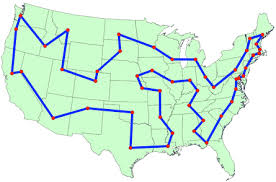
\includegraphics[width= 0.5\textwidth]{figures/tspexample.jpg} 
    \caption[TSP solved instance of USA capitals]{TSP solved instance of USA capitals}
    \label{fig:flow around cylinder} 
\end{figure} 

Travelling Salesman Problem takes its name from one of its natural application: the
the problem of a traveling salesman who has to pass through all the cities he has to
visit only once and efficiently. In a more formal description, TSP solves the following
problem: given n points and a metric function to define costs between all the pair
of node, the goal is to find a path starting and ending in the same node and passing
through all the other exactly once. To be more precise, the fact that exists a path
between every pair of nodes is a restriction of the original problem and, combined
with the fact that the distances between nodes follow the euclidean distance, we
can talk about \emph{Euclidean TSP}.

TSP belongs to the class of the NP-Hard problem and it has been for many decades
a benchmark for several innovative ideas and heuristics. For this reason,
throughout the years, the goal to solve those larger TSP instances became a
challenge for all the computer scientist. In the early 50s, the known models
could only find a solution for the problem of around 50
nodes\citep{dantzig1954solution}. In 1987 this limit grew firstly to 532 and
then to 2392. It took another 17 years to reach the goal of almost 25000 node
instances with some intermediate improvements.

\begin{table}[H] 
    \centering 
    \begin{tabular}{c|c}
        Year & Nodes \\
        1954 & 49 \\
        1971 & 64 \\
        1977 & 120 \\
        1980 & 318 \\
        1987 & 532 \\
        1987 & 2392 \\
        1994 & 7397 \\
        1998 & 13509 \\
        2004 & 24978 
    \end{tabular} 
    \caption{Solved instances milestones} 
\end{table}

For its intrinsic complexity during years a lot of approximation algorithm has
been proposed to try to achieve a good resolution in polynomial time. The first
good results in terms of approximation guaranteed a $2$-approximation solution
using a simple spanning tree technique. It has been later refined by the known
Christofides algorithm that led to a $\frac{3}{2}$-approximation using similar
ideas. However, even if it is theoretically better its results are not so
different, and being computational more demanding it is not always considered
as the best trade-off. After a very long time from these results, last year, a
paper has been presented claiming that it is possible to lower the Christofides
bound on the approximation.

\section{Mathematical Model}

If the goal aims to find the optimal solution the best know ways to do it is
using integer linear programming. TSP, in fact, can be translated into an ILP
model quite simply. The constraints ruling the model depend on the fact that
each node has to be visited and it has to be reachable from the starting one.
TSP can be formulated as a symmetric or asymmetric problem depending on the
initial requirements. The original graph-related problem, in fact, can be
expressed in both ways. However, the symmetric version of the problem can be
seen as a particular instance of the asymmetric one where from an arc two are
created having the same cost and opposite directions. For this reason, in this
introduction, we deal with the asymmetric problem.

Let now see the formal definition of the model. 

Be $G = (V, A)$ the graph for which $V$ is the set of vertices and $A$ the set
of arcs for each is defined the parameter $c_{ij},\ (i,j) \in A$ as the cost on
arc $(i,j)$.

To solve the problem new binary variables $x_{ij}$,\ $(i,j) \in A,\ i \neq j$
determines whether an arc $(i,j)$ has to be selected as being part of the tour.

\begin{equation*}
    \begin{array}{lrllr}
        \textrm{minimize}   & \displaystyle\sum_{(i, j) \in A} c_{ij}  x_{ij} \\
        \textrm{subject to} & \displaystyle\sum\limits_{(i, j) \in \delta^-(j)}  x_{ij} & = & 1 & \forall j \in V\\
                            & \displaystyle\sum\limits_{(i, j) \in \delta^+(i)}  x_{ij} & = & 1 & \forall i \in V\\
                            & \displaystyle\sum\limits_{(i, j) \in \delta^+(S)}  x_{ij} & \ge & 1 & \forall S \subset V : 1 \in S\\
                            & x_{ij} & \in & \{0,1\} & \forall (i,j) \in A \\
    \end{array}
\end{equation*}


The objective function aims to minimize the total cost of the solution. The
model is subject to three constraints. The first imposes that every node is
reached by an arch so it means the node is visited. The second one guarantees
that the path leaves the node so given the first constraint it means that the
path involving that node is going to be a cycle.

In the symmetric version, these two constraints can be merged into a single one
defined as
\begin{align*} 
    \sum_{(i,j) \in \delta(i)} x_{ij} & = 2 & \forall i\in V
\end{align*} 
However, even if it could seem enough, there is the need to ensure that the
model creates a single path starting and ending in the initial node. For this
reason, we impose reachability from 1 constraint, aka subtour elimination
constraint, which prevents subtours (which don't involve 1) to form. The SEC
can be also expressed in this way:
\begin{align*} 
    \sum_{i,j \in S,\ i \neq j} x_{ij} & \le |S|-1 & \forall S \subset V: |S| \ge 2
\end{align*}
that explicitly express to eliminate subtours.
The formulation above is easy to write in a solver and it is correct, but it
presents a big issue. While the degree constraints are in a linear number with
respect to the number of nodes, the subtour elimination constraints in the
basic formulation are exponential and so not feasible to apply in practice. New
formulation of these constraint have made possible to deal with larger and
larger instances and in this thesis we are going to show some of these ideas
and other heuristic that made TSP feasible for significant instances.


% Related work 
\chapter{Compact Models}
In the introduction, we left the mathematical model with an open problem: the
number of the subtour elimination constraints made infeasible the
implementation. Recalling the model we have shown before you can notice that
the variables are $\frac{n(n-1)}{2}$ and the number of constraints is
exponential because we have one subtour for almost any subset of nodes. Even if
the solution proposed in 1954 by Dantzig, Fulkerson and Johnson has been a
milestone in the history of the problem it could only solve an instance of 49
nodes. In the following years, new ways to eliminate the subtours were found
using only a linear (polynomial, in general) number of constraints. In this
chapter, we will discuss two of the most important formulations of these
compact models, build on the asymmetric version of the problem.

\section{Miller-Tucker-Zemlin}
The \emph{Miller-Tucker-Zemlin} model
\citep{miller1960integer}\citep{sawik2016note} (MTZ from now on) is defined as a
sequential formulation and it is because that the idea upon the model is to
introduce a new continuous variable $u_i$ for each node $i \in V \setminus
\{1\}$ (except the starting node). The meaning behind these $u$ variables is
to represent the order of visit of the nodes considering an optimal tour. It's
possible to define such an order because the asymmetric version of the problem
is considered. An example of such new variables is shown in figure
\ref{fig:MTZ_example}.

\begin{figure}
    \centering
    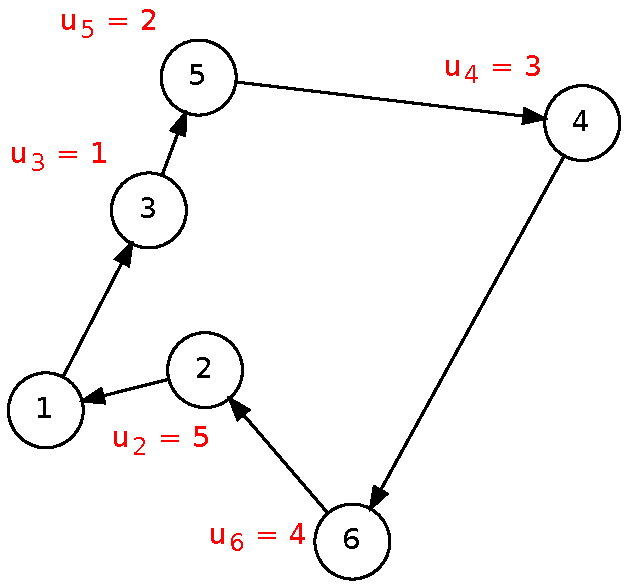
\includegraphics[width=0.43\textwidth]{figures/mtz}
    \caption[MTZ example]{Variables $u$ represent the tour visit order}
    \label{fig:MTZ_example}
\end{figure}

Given the arc $x_{ij}$ selected for the tour, the tour visit can be expressed
as $u_j \geq u_i + 1$. In symbols:


\begin{equation*} 
    \begin{array}{llr} 
        x_{ij} = 1 \implies & u_j \geq u_i + 1 & \forall i, j \in V \setminus \{1\},\ i \neq j \\
                            & u_i \in \{1, \dots\ n-1\} & \forall i \in V \setminus \{1\}
    \end{array} 
\end{equation*}

this will prevent the formation of subtours. 
The constraint is modeled as a
logic implication, but it is possible to define it also using \emph{big-M}
formulation, where the implication is dropped in favor of a modified right-hand
side that activates the constraint depending on the value of $x_{ij}$.

\begin{equation*} 
    \begin{array}{lr} 
        u_j \geq u_i + 1 \textcolor{red}{ - M (1 - x_{ij})} & \forall i, j \in V \setminus \{1\},\ i \neq j \\
    \end{array} 
\end{equation*}

that can be rewritten as

\begin{equation*} 
    \begin{array}{lr} 
        u_i - u_j + M x_{ij} \leq M - 1 & \forall i, j \in V \setminus \{1\},\ i \neq j \\
    \end{array} 
\end{equation*}

The bounds on $u$ variables remain unaltered. $M$ is supposed to be a
value large enough to trivially truly evaluate the inequality if the arc is not
selected and considering the bounds on $u$ variables, but tight enough to
prevent numerical difficulties
\footnote{\href{https://www.ibm.com/docs/en/icos/20.1.0?topic=optimization-best-practices-indicator-constraints}{https://www.ibm.com/docs/en/icos/20.1.0?topic=optimization-best-practices-indicator-constraints}}.
The smallest (and best) value for $M$ considering the formulation is $n - 1$.

\subsection{Miller-Tucker-Zemlin model}
\begin{equation*}
    \begin{array}{lrllr}
        \textrm{minimize}   & \displaystyle\sum_{(i, j) \in A} c_{ij}  x_{ij} \\
        \textrm{subject to} & \displaystyle\sum\limits_{(i, j) \in \delta^-(j)}  x_{ij} & = & 1 & \forall j \in V\\
                            & \displaystyle\sum\limits_{(i, j) \in \delta^+(i)}  x_{ij} & = & 1 & \forall i \in V\\
                            & x_{ij} & \in & \{0,1\} & \forall (i,j) \in A \\ \\
                            & u_i - u_j + (n-1) x_{ij} & \leq & n - 2 & \forall i, j \in V \setminus \{1\},\ i \neq j \\
                            & u_i & \in & \{1,\ \dots n-1\} & \forall i \in V \setminus \{1\}
    \end{array}
\end{equation*}

We have to verify that any tour in which node 1 is not present violates the
constraint and that the tour with node 1 does not. It would led to a solution
with only one complete tour. 
We first deal with a subtour of $k$ elements not passing through node 1.

\begin{theorem} 
    Given the two degree constraints, the inequalities $u_{i} -
    u_{j} + (n-1) x_{ij} \le n-2$ $\forall i,j\in V \setminus \{1\}, i\neq j$
    guarantee that the final solution contains a tour passing through node 
    $\{1\}$ and no tours not passing through it. 
\end{theorem}

\begin{proof}
    First, prove that for any tour that not contains the starting node at least
    one of the inequalities is violated by a pair of nodes of the tour. To show
    that it is enough to sum all the constraints relative to the selected arcs.
    All u variables are summed and subtracted once. Hence the sum of the $k$
    (number of nodes in the tour) constraints will end up in an impossible
    inequality $k(n - 1) \leq k(n - 2)$. Since we know that given the degree
    constraints the solution does not contain an open path and we just saw that
    there are no tours that do not pass through the source node, it is
    sufficient to show that a tour passing through 1 can exist to prove that
    the solution returns a Hamiltonian circuit. To show that it is enough to
    verify if single constraints are violated both in case arcs are selected or
    not. For $x_{ij} = 0$ it is straightforward because $u_i - u_j \leq n - 2$
    since $u_i \leq n - 1$ and $u_j \geq 1$. Being u position variable we can
    define their value as the discrete-time $t$ in which they are visited. So
    assuming $x_{ij} = 1$ the node $i$ is visited immediately before than $j$
    so if $u_i = t$ then we can assume $u_j = t + 1$. In this way constraint is
    satisfied since $u_i - u_j + n - 1 \leq n - 2 \implies t - (t + 1) + n - 1
    \leq n - 2$ that is valid because $t - (t + 1) + n - 1 = -1 + n - 1 = n -
    2$.
\end{proof}

\subsection{CPLEX implementations}
MTZ implementation using CPLEX can be done using different techniques. Besides
the straightforward implementation of the degree constraints, MTZ's subtour
elimination constraints can be implemented in different ways. \\ One of CPLEX's
features are \emph{indicator
constraints}\footnote{\href{https://www.ibm.com/docs/en/icos/12.9.0?topic=optimization-what-is-indicator-constraint}{https://www.ibm.com/docs/en/icos/12.9.0?topic=optimization-what-is-indicator-constraint}},
a way to activate or not a certain constraint depending on the value of a
control, binary variable. Internally this is implemented with big-M technique or
through local activation of that constraint in a certain node during
branching, while that variable is fixed. This is the perfect scenario for the
first version of MTZ SECs we presented. \\ 
The other way, the one we presented in the model, uses big-M formulation, which
implementation is straightforward. We will refer to this as the \emph{static}
model. \\
Another possibility is using \emph{lazy constraints}
\footnote{\href{https://www.ibm.com/docs/en/icos/12.9.0?topic=pools-what-are-user-cuts-lazy-constraints}{https://www.ibm.com/docs/en/icos/12.9.0?topic=pools-what-are-user-cuts-lazy-constraints}}
, a type of constraints that are not immediately added to the model, but
activated once they are necessary. The idea behind this is to specify as lazy
some constraints that are unlikely to be violated, keeping the model thinner.
Again, a perfect scenario for our big-M SECs. We will refer to this as the
\emph{lazy} model. They have some limitations, the most notable is that a lazy
constraint cannot have indicator constraints, so we cannot mix the two
implementations. 

\begin{claim}
    The best implementation is the one that takes advantage of lazy constraints.
\end{claim}

\begin{figure}
    \centering
    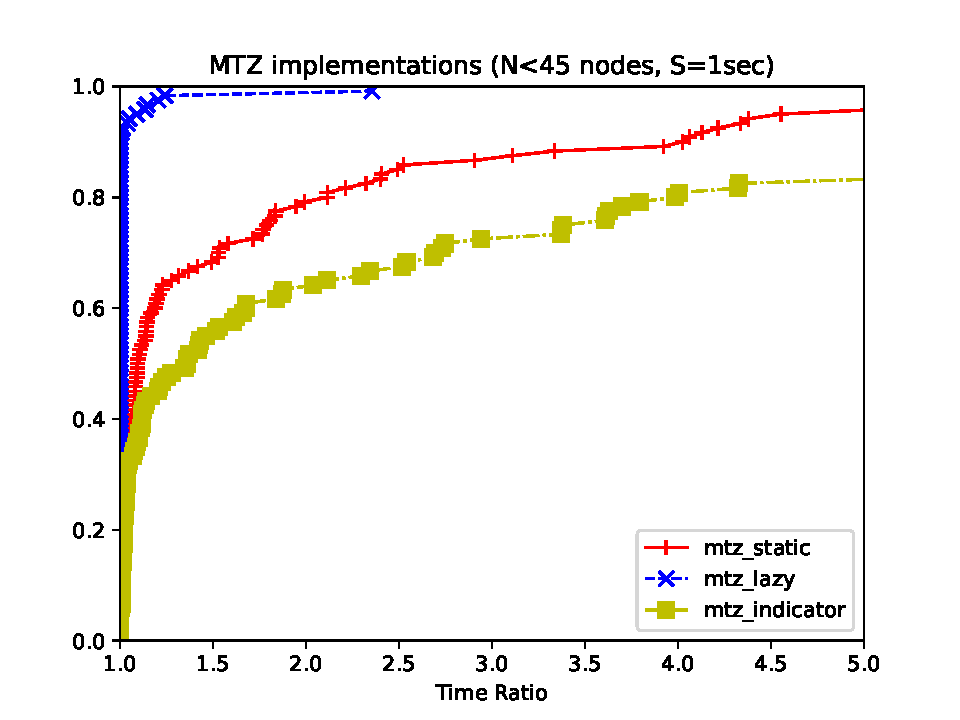
\includegraphics[width=0.8\textwidth]{figures/mtz_comp1.pdf}
    \caption{MTZ implementations comparison}
\end{figure}

The graph is representing the result of geometric-mean profiler
\citep{dolan2002benchmarking}. A total of 120 instances are tested, 30 of which
are around 45 nodes (that will ensure a $<10$ min execution time). More on
testing setup and parameters settings in appendix \ref{appendix:testenv}. \\

The result of the benchmark is pretty clear: the model implemented through lazy
constraints is faster than the other two. We can also assert that the static
model is faster than the one which uses indicator constraints.\\
Since the results allow us to and bearing in mind that correlation does not
imply causality, we can carefully assert that the smallness of the model makes
it faster. This is true if lots of constraints are not violated (then not added to the
model), while on the static all of the constraints are present at starting time.
This is also true considering the static model versus the one with indicator
constraints, which is a comparison between formulations. In fact, after an
analysis of CPLEX logs, it is possible to notice that the presolve didn't reduce
the model size with indicators, which has always more rows and more columns (in
general, more non-zeroes) than the static model. 

\begin{table}[h]
    \begin{tabular}{rl}
    \begin{tabular}[c]{@{}r@{}}Static\\ log\end{tabular}    & \begin{tabular}[c]{@{}l@{}}\footnotesize \texttt{Reduced MIP has 977 rows, 675 columns, and 3750 nonzeros.}\\ \footnotesize \texttt{Reduced MIP has 650 binaries, 25 generals, 0 SOSs, and 0 indicators.}\\ \footnotesize \texttt{...}\end{tabular} \\
    \begin{tabular}[c]{@{}r@{}}Indicator\\ log\end{tabular} & \begin{tabular}[c]{@{}l@{}}\footnotesize \texttt{Reduced MIP has 1277 rows, 975 columns, and 4050 nonzeros}.\\ \footnotesize \texttt{Reduced MIP has 650 binaries, 25 generals, 0 SOSs, and 600 indicators.}\\ \footnotesize \texttt{...}\end{tabular}                          
    \end{tabular}
    \caption[MTZ size comparison on indicator versus static model]{\centering Model size for toy example of 26 nodes. There are $300 =
    \frac{600}{2} = \frac12 2 {25 \choose 2}$ non-zeroes, rows and columns with respect to the static model}

\end{table}

In fact, for all three model sizes (rows, cols and non-zeroes) the indicator has
exactly half of the number of SECs in addition to the others. This is true for
rows and non-zeroes, while for columns, the number of variable in the static model
plus half of the number of SECs is reported in the model size section, while in
the section that exploits the nature of the variables, all of the variables in
the static one are reported, in addition to others marked as \emph{indicators}
(equal to the number of SECs). Keeping in mind that the number of SECs is $2 \cdot
{ n \choose 2} = 2 \cdot \frac{n (n - 1)}{2} \in \mathcal{O}(n^2)$, this result
cannot be ignored. Another important fact to analyze is that the presolve on the
lazy model worked really well: it drastically reduced the number of rows,
probably the key to the success of this formulation.\\

Considering how the indicator constraints are well sold on CPLEX
guidelines\footnote{\href{https://www.ibm.com/support/pages/node/397209}{https://www.ibm.com/support/pages/node/397209}},
the results are kinda surprising. But the guidelines state also that a big-M
formulation should be avoided when M is much larger than any other coefficient
and when the model does not suffer from big-M side effects (numerical issues,
mainly), that is not our case. We precisely choose $M$ and set the
parameter \texttt{CPX\_PARAM\_EPINT} to ensure general correctness. We suppose
that those advice on indicator constraints are given to prevent a poor choice
of $M$ and, consequently, a hard time debugging numerical issues, which can be
difficult to exploits.

\subsection{Speeding up the model}
The model we presented is correct, in the sense that solves the problem for a
reasonable amount of time up to a certain number of nodes. The performance of
the model, however, can be improved by adding some constraints that tight the LP
relaxation during branching. The constraints we're up to adding are SECs from
Dantzig, Fulkerson and Johnson formulation, restricted to a certain size of
subsets. The problem with that formulation is that the total number of
constraint is exponential in $n$, but the idea is to add only those constraints
that involve subsets of nodes of size 2 or at most 3.\\

We will refer as \emph{SECs of degreee 2} this constraints:

\begin{equation*} 
    \begin{array}{lr} 
        x_{ij} + x_{ji} \leq 1 & \forall i, j \in V,\ i \neq j
    \end{array} 
\end{equation*}

and as \emph{SECs of degreee 3}:

\begin{equation*} 
    \begin{array}{lr} 
        x_{ij} + x_{jk} + x_{ki} \leq 2 & \forall i, j, k \in V,\ i \neq j \neq k
    \end{array} 
\end{equation*}

This will prevent subtours of size 2 and size 3 to form. We have to keep in mind
that the total number of constraints added is not that negligible: for degree 2
SECs they are ${n \choose 2} \in \mathcal{O}(n^2)$ while for degree 3 they are
$2 \cdot {n \choose 3} \in \mathcal{O}(n^3)$. Note that for degree 3, we have to
consider both circular paths due to asymmetry (for example, considering node 2,
5 and 8, we have to add both $x_{25} + x_{58} + x_{85} \leq 2$ and $x_{28} +
x_{85} + x_{52} \leq 2$). Clearly, does not exist such degree 1 SECs because
self-loops are not allowed in the model.

The idea is to add only a small amount of constraint so the model is still
compact but powerful enough to speed up the branching process. We have to find a
trade-off for this. We can consider degree-2 constraints as a correction of the
asymmetric model with respect to the symmetric one: because of asymmetry, we
have double the number of variables, because an edge is converted in two arcs.
A degree-2 constraint for a couple of arcs means that if one of them is fixed,
also the other one had to be fixed, so we don't have freedom of choice on the
other one, exactly as the symmetric version (because there's only one edge!).
The ovehead is to have twice the variables and specialized constraints to manage
this behavior.

\begin{claim} 
    The solve time for MTZ model can be improved including deegree-2 subtour
    elimination constraints. 
\end{claim}

\begin{figure}[h]
    \centering
    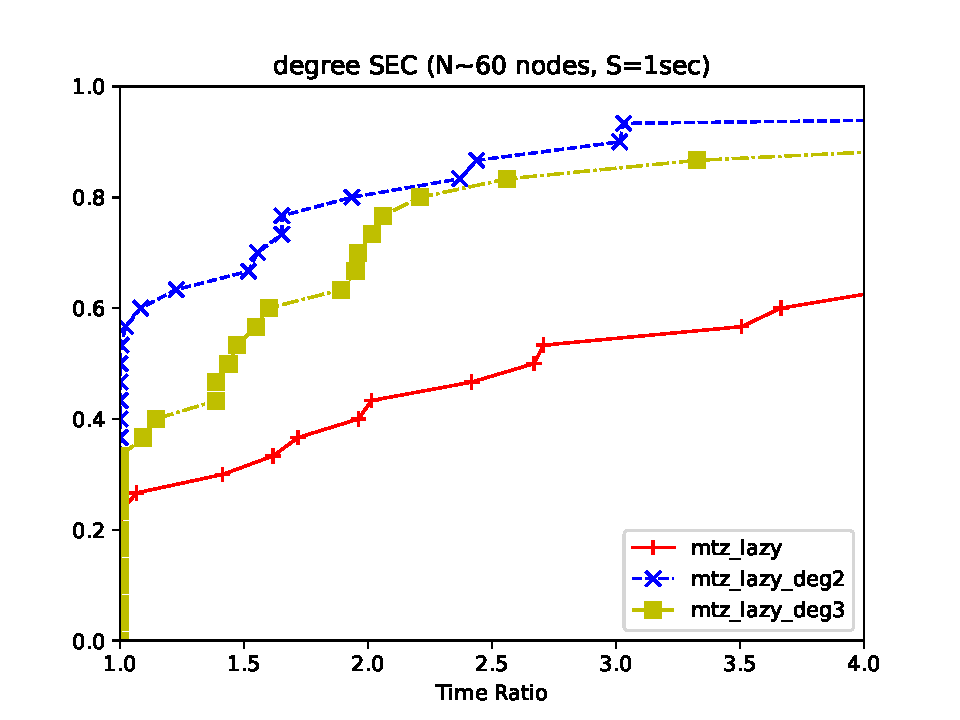
\includegraphics[width=0.8\textwidth]{figures/mtz_comp2.pdf}
    \caption{MTZ degree SECs comparison}
\end{figure}

The comparison is done on lazy implementation (because of it's superior with
respect to the others) so the number of nodes for istance can be increased to
avoid any bias: 30 istances of ~60 nodes are tested.\\

The graph shows the superiority of degree 2 SECs model with respect to a basic
implementation and to degre 3 SECs model (which includes both constraints of
degree 2 and 3). This is probably due to the number of constraints added that,
despite being lazy, they're too much considering the degree 3 model. As
we could expect, the degree 3 model works pretty well when the model is small
or easy to solve, because the total number of constraints added is not so
different than the degree 2 model. Considering that the goal is to solve
efficiently hard problems, this information is not that interesting.

\subparagraph{Note:} claim 1 was produced considering adding all the degree
2 Danzing's subtour elimination constraints. Overall, we can consider the big-M
formulation with degree 2 SECs and implemented using lazy constraints as the
winner over all possible MTZ formulations and implementations.




\section{Gavish and Graves}
In 1978 Gavish and Graves \citep{gavish1978travelling}\citep{orman2006survey}
proposed an alternative solution based on a flow idea. This method introduces a
variable $y_{ij}$ for each arc $(i,j) \in A,\ (i\neq j)$, which represents the
\emph{quantity of flow} in the arc. The source of the flow is node 1, and its
destination after visiting the graph. Starting at its maximum capacity ($n -
1$) the flow loses one unit each time it visits a node, returning to node 1
with no flow at all. Figure \ref{fig:GG_example} shows the idea in a toy
example.

\begin{figure}[h]
    \centering
    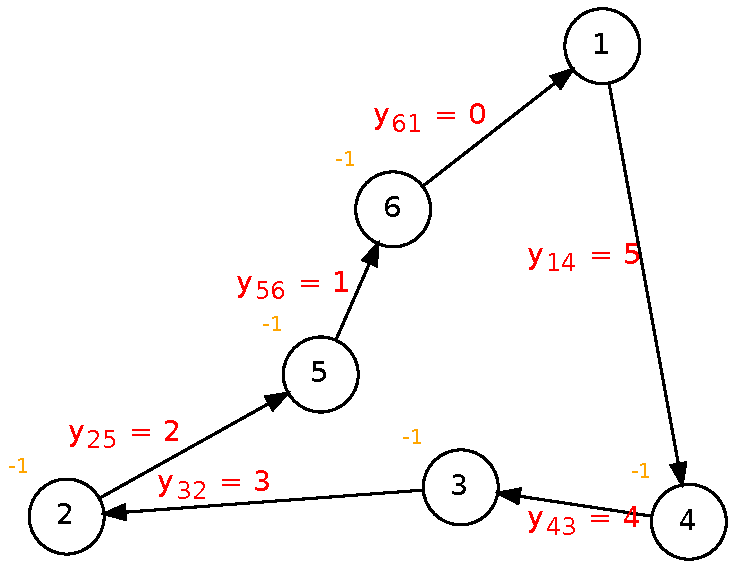
\includegraphics[width=0.43\textwidth]{figures/gg}
    \caption[GG example]{Variables $y$ represent flow quantity}
    \label{fig:GG_example}
\end{figure}

First of all, we have to model the flow. We have to model the flow at the
beginning, as well at the end, and its behavior during the visit.
Respectively, they are modeled with

\begin{equation*} 
    \begin{array}{rrlr} 
        y_{1j} & = & (n - 1) x_{1j} & \forall j \in V \setminus \{1\} \\
        y_{i1} & = & 0 &\forall j \in V \setminus \{1\} \\
        \underbrace{\displaystyle\sum\limits_{i = 1, i \neq h}^n y_{ih}}_{in-flow\ node\ h} & = & \underbrace{\displaystyle\sum\limits_{j = 1, j \neq h}^n y_{hj}}_{out-flow\ node\ h} + 1 & \forall h \in V \setminus \{1\}\\
    \end{array} 
\end{equation*}

We will refer to them as \emph{flow-model constraints}. The first one model the
out flow from node 1, which has to be set at its maximum capacity, $n - 1$.
Only one of the $x_{1j},\ j \in V \setminus \{1\}$ will be set to one so, for
that arc, the flow will be $n - 1$.\\ The second one model the in flow at node
1, which is zero, because we are supposing that during the visit of the remain
$n - 1$ nodes, the flow will decrease to zero. Notice that we can model this
constraint imposing a different upper bound to those variables: these
constraints will be dropped from the model during implementation.\\ The third
one model the leaking of one flow quantity during each visit that not involves
node 1.\\
The last thing to do is to link the flow variables to the arc selection
variables, so if an arc is selected, the flow is free to pass through it. We
can model this imposing different upper bound on flow capacity for that arc:

\begin{equation*} 
    \begin{array}{rlrr} 
        x_{ij} = 0 \implies & y_{ij} = 0 & \forall i, j \in V \setminus \{1\},\ i \neq j \\
        x_{ij} = 1 \implies & y_{ij} = n - 2 & \forall i, j \in V \setminus \{1\},\ i \neq j \\
    \end{array} 
\end{equation*}

this logical implication can be modeled as

\begin{equation*} 
    \begin{array}{rrlr} 
        y_{ij} & \leq & (n - 2) x_{ij} & \forall i, j \in V \setminus \{1\},\ i \neq j \\
    \end{array} 
\end{equation*}

We will refer to them as \emph{linking constraints}. It is possible to notice
that the in/out flow from node 1 are a special case of this constraint, in
fact, this one imposes an $n - 2$ upper bound on the value of $y_{ij}$ because
that case is already managed, and the bound can be made tighter.\\
The bound on the variables are simply

\begin{equation*} 
    \begin{array}{rrlr} 
        y_{ij} & \in & \{0,\ \dots n-1\} & \forall i,j \in V,\ i \neq j
    \end{array} 
\end{equation*}

this works in general, but on the implementation side, the bounds can be
restricted at $n - 2$ for all nodes different from 1 and to $0$ for the in-flow
variable at node 1, as previously mentioned. It's interesting to note that the 
variables are not necessarly integers, but providing such information to the
solver is always a good practice.\\ 
Since this formulation was presented in class, we will refer to
it as \emph{lecture model}, which is summarised below:

\subsection{Gavish-Graves model, lecture}
\begin{equation*}
    \begin{array}{lrllr}
        \textrm{minimize}   & \displaystyle\sum_{(i, j) \in A} c_{ij}  x_{ij} \\
        \textrm{subject to} & \displaystyle\sum\limits_{(i, j) \in \delta^-(j)}  x_{ij} & = & 1 & \forall j \in V\\
                            & \displaystyle\sum\limits_{(i, j) \in \delta^+(i)}  x_{ij} & = & 1 & \forall i \in V\\
                            & x_{ij} & \in & \{0,1\} & \forall (i,j) \in A \\ \\
                            & \displaystyle\sum\limits_{i = 1, i \neq h}^n y_{ih} & = & \displaystyle\sum\limits_{j = 1, j \neq h}^n y_{hj} + 1 & \forall h \in V \setminus \{1\}\\
                            & y_{1j} & = & (n - 1) x_{1j} & \forall j \in V \setminus \{1\} \\
                            & y_{i1} & = & 0 & \forall j \in V \setminus \{1\} \\
                            & y_{ij} & \leq & (n - 2) x_{ij} & \forall i, j \in V \setminus \{1\},\ i \neq j \\
                            & y_{ij} & \in & \{0,\ \dots n-1\} & \forall i,j \in V,\ i \neq j
    \end{array}
\end{equation*}

Even if this model is correct, it is possible to modify it while keeping
correctness. The in-flow contraints for node 1 are implicitly satisfied
considering the initial value of the flow and the fact that the flow loses one
quantity for each visit (modeled by the flow control constraints). Anyway, this
is no big deal considering that those constraints were implemented as variable
bounds.\\ The out flow constraints from node 1 can be merged in this one:

\begin{equation*} 
    \begin{array}{rrlr} 
        \displaystyle\sum\limits_{j = 1, j \neq 1}^n y_{1j} & = & n - 1 & \\
    \end{array} 
\end{equation*}

\newpage
Clearly, just one element of the sum will be equal to $n - 1$: considering the
flow loss, lenght of tour and variable bounds, the flow has to start with that
value.\\ 
We still need to link the selection of an arc starting from node 1 to
the full capacity on that arc, made possible by 

\begin{equation*} 
    \begin{array}{rrlr} 
        y_{1j} & \leq & (n - 1) x_{1j} & \forall j \in V \setminus \{1\} \\
    \end{array} 
\end{equation*}

which can be seen as a specialized case of linking constraints for node 1. The
remaining linking constraints, as well as flow-model constaints, remains
unaltered.
Since this model is the most frequent in literature, we will refer to it as
\emph{literature model}, which is summarised below:

\subsection{Gavish-Graves model, literature}
\begin{equation*}
    \begin{array}{lrllr}
        \textrm{minimize}   & \displaystyle\sum_{(i, j) \in A} c_{ij}  x_{ij} \\
        \textrm{subject to} & \displaystyle\sum\limits_{(i, j) \in \delta^-(j)}  x_{ij} & = & 1 & \forall j \in V\\
                            & \displaystyle\sum\limits_{(i, j) \in \delta^+(i)}  x_{ij} & = & 1 & \forall i \in V\\
                            & x_{ij} & \in & \{0,1\} & \forall (i,j) \in A \\ \\
                            & \displaystyle\sum\limits_{i = 1, i \neq h}^n y_{ih} & = & \displaystyle\sum\limits_{j = 1, j \neq h}^n y_{hj} + 1 & \forall h \in V \setminus \{1\}\\
                            & \displaystyle\sum\limits_{j = 1, j \neq 1}^n y_{1j} & = & n - 1 & \\
                            & y_{ij} & \leq & (n - 2) x_{ij} & \forall i, j \in V \setminus \{1\},\ i \neq j \wedge i \neq 1 \\
                            & y_{1j} & \leq & (n - 1) x_{1j} & \forall j \in V \setminus \{1\} \\
                            & y_{ij} & \in & \{0,\ \dots n-1\} & \forall i,j \in V, i \neq j
    \end{array}
\end{equation*}

\subsection{CPLEX implementations}
Both formulation allows an implementation that uses lazy constraints, so
everything will be tested. The model, anyway, it's different from MTZ by the
number of variables, which is $\mathcal{O}(n^2)$. If we exclude
SECs of degree 2, the model is bigger than MTZ, but still compact.

\begin{claim} 
    The best combination of formulation and implementation is the literature
    model implemented through static constraints. 
\end{claim}

\begin{figure}[h]
    \centering
    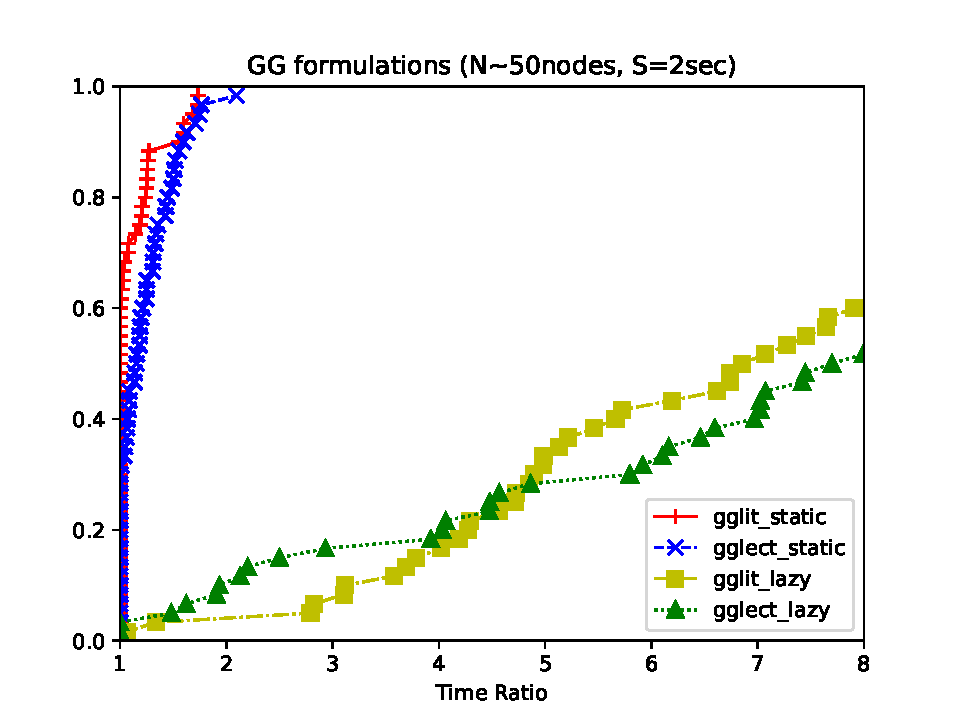
\includegraphics[width=0.8\textwidth]{figures/gg_comp1}
    \caption{GG formulations and implementations comparison}
\end{figure}

The comparison is done considering 60 instances of around 50 nodes each. It's
clear that the static implementation is better than the lazy one. Recall that
the main idea behind lazy constraints is to add them only when needed, keeping
the model small for relaxations. They are supposed to be violated very few
times, but this is not the case. The GG SECs models a behavior of lots of
variables ($\mathcal{O}(n^2)$), so it's expected that will be a lot of
constraints violated. We tested the number of constraint violation (during whole
execution) by running the lazy implementations of MTZ and GG (both formulations)
on a total of 25 instances (5 of which composed of 10 ,20, 30, 40 and 50
nodes).

\begin{figure}[h]
    \centering
    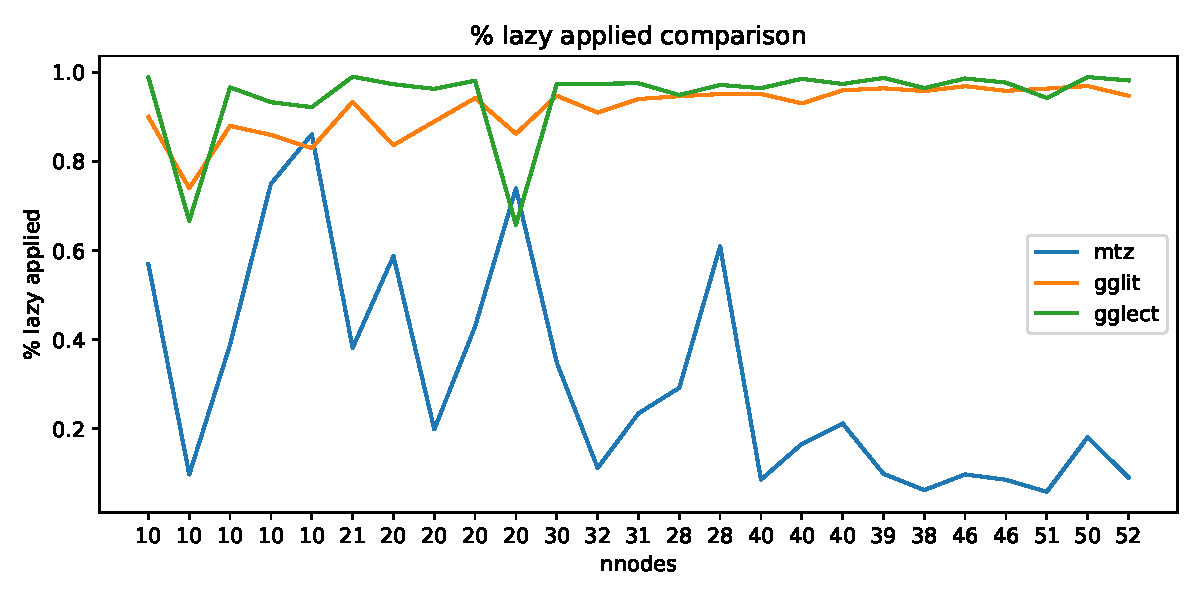
\includegraphics[width=0.78\textwidth]{figures/perc_lazy}
    \caption{Percentage of lazy violations for each model}
\end{figure}

While keeping in mind that the number of constraints is quadratic in number of
nodes, we can observe that the number of lazy violations in MTZ (blue line) is
decreasing (and independent in the number of nodes) so, roughly, constant in
absolute values, while in both formulation of GG  (orange and green lines),
almost all constraints are violated. That makes the implementation through lazy
constraints ideal for MTZ and costrly for GG, because of model reshapes during
executions.\\

Both static models are quite good, with the literature formulation that performs
slightly better that the one presented in class.


One may ask if the Dantzig's SECs for degree 2 that worked beautifully in the MTZ
model could also help here.

\begin{claim} 
    The solve time for GG model can be improved including deegree-2 subtour
    elimination constraints.
\end{claim}

We tested the best model in the previous comparison, the literature formulation
with static constraint, statically adding the additional SECs. We tested 30
instances of 80 nodes each.

\begin{figure}[h]
    \centering
    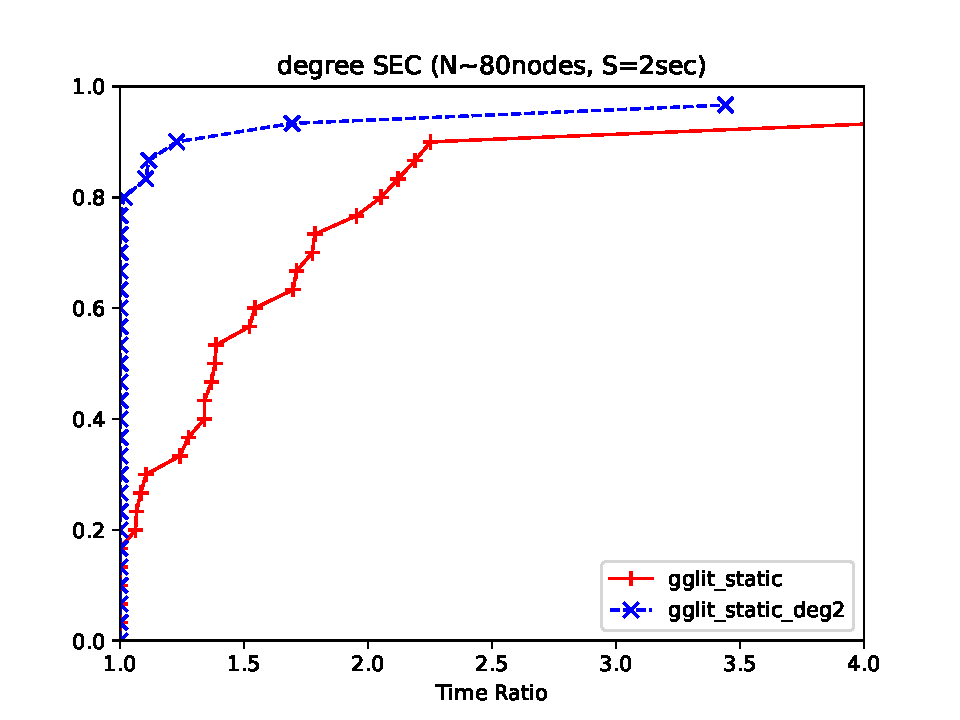
\includegraphics[width=0.8\textwidth]{figures/gg_comp2}
    \caption{GG degree SECs comparison}
\end{figure}

The answer is positive, those constaints are helpful also here. \\ 

The static implementation of the literature formulation with degree-2 SECs
is the winener among all possible formulations and implementations.

\section{Compact models comparison}
Finally, we tested MTZ agains GG, considering for both of them the optimal
formulation / implementation on a test bed of 30 instances of 80 nodes.

\begin{claim} 
    GG is a better compact model formulation of TSP compared with MTZ.
\end{claim}

\begin{figure}[h]
    \centering
    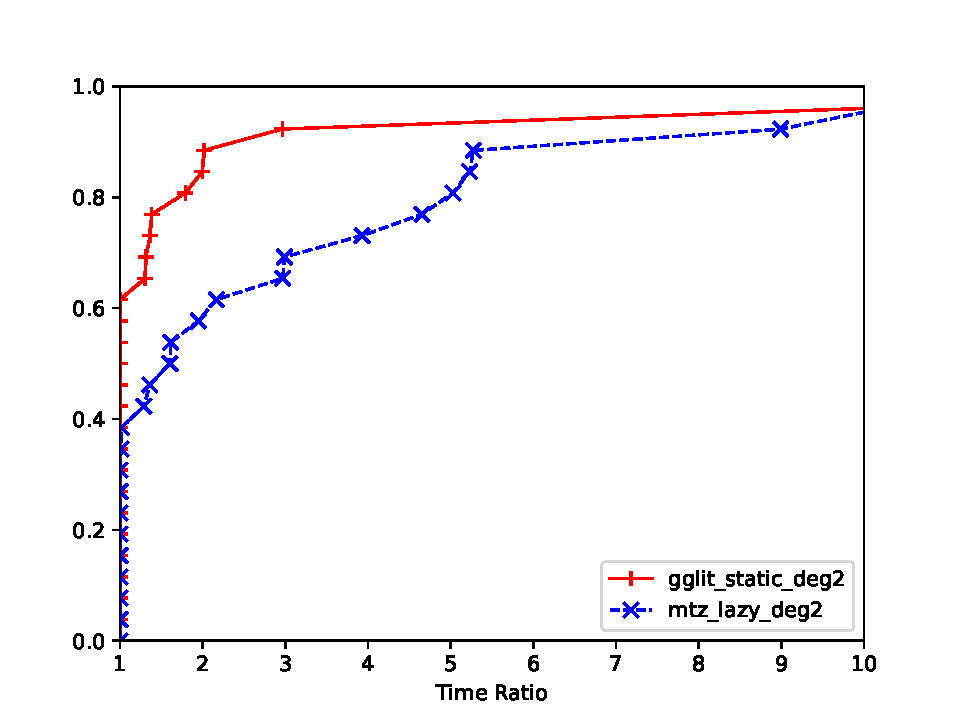
\includegraphics[width=0.8\textwidth]{figures/compact_final}
    \caption{Compact models comparison}
\end{figure}

We can decree the Gavish and Graves as the best compact model for euclidean TSP.
It's nice to notice that, give a fixed time limit, the number of nodes solved to
optimality in that timelimit act as a benchmark for the performance of the
methods and approaches to TSP. In this case, considering our setup, 80 nodes is
the maximum amount that can be solved by limiting the computation to 10 minutes.
It's also important to check each time that the solutions obtained are optimal,
in the sense that if one of the two methods reaches time limit, the beast
feasible solution obtained during branch-and-cut is obtained, but there's a loss
of sense to compare it with the other solution produced by the other method. In
our tests, we will ensure that all this details are taken into consideraiton.


\chapter{Benders Method}
\section{The Loop method}
Compact models are an efficient way to model the TSP with a polynomial number of
constraints. However, they allow solving only small instances since they still
have a huge number of them. A more efficient way to avoid subtours would be to
generate the subtour elimination constraints on the fly, only when needed while
precisely targeting a subtour elimination.\\
Benders method is a general strategy to solve MIP problems: it starts solving a
reduced version of the model (in which some constraints, even those that ensures
correctness, are relaxed) and then it adds to the model that constraints that
would be violated (according to actual solution) if present from the beginning.
Then it repeats the procedure until a correct solution is obtained.\\
Applied to TSP: we start from an SEC-free model that will produce subtours, we
solve it using a MIP solver as a black box until we found a solution with
subtours. For each of them, we have to add to the model Danzing's SEC: this will
prevent those subtour to form the next iteration. We repeat this until a
single-tour solution is obtained.

\begin{algorithm}[H]
\SetAlgoLined
\KwResult{A subtour-free solution}
    \emph{model} $\leftarrow$ prepare SEC-free model\;
    \emph{sol} $\leftarrow$ MIP opt (\emph{model})\;
    \While{sol contains subtours}{
        \ForEach{subtour s in sol} {
            add to \emph{model} Danzing's SEC that involves $s$
        }
        \emph{sol} $\leftarrow$ MIP opt (\emph{model})
    }
    \caption{The Loop method}
\end{algorithm}

Since it uses a MIP solver as a black box inside a loop, we will refer to it as
the \emph{Loop method} or, improperly since it is its generalization,
\emph{Benders method}.

There's no reason to use an asymmetric version of the problem, the symmetric one will works well. Danzing's SEC
that will be added at each iteration became:

\begin{equation*} 
    \begin{array}{rrlr} 
        \displaystyle\sum_{i,j \in S,\ i \neq j} x_{ij} & \le |S|-1 & \forall S \subset V: |S| \ge 3
    \end{array} 
\end{equation*}

Notice that the number of non-zero on the left-hand side of the constraint is
${|S|\choose 2} \in \mathcal{O}(|S|^2)$ and that we are considering subset $S$
of at least dimension 3: for dimension 2 the constraint is clearly absorbed in
the variable's bounds ($x_{ij} \le 1$).

\begin{figure}[h]
    \centering
    \begin{minipage}{.45\textwidth}
        \centering
        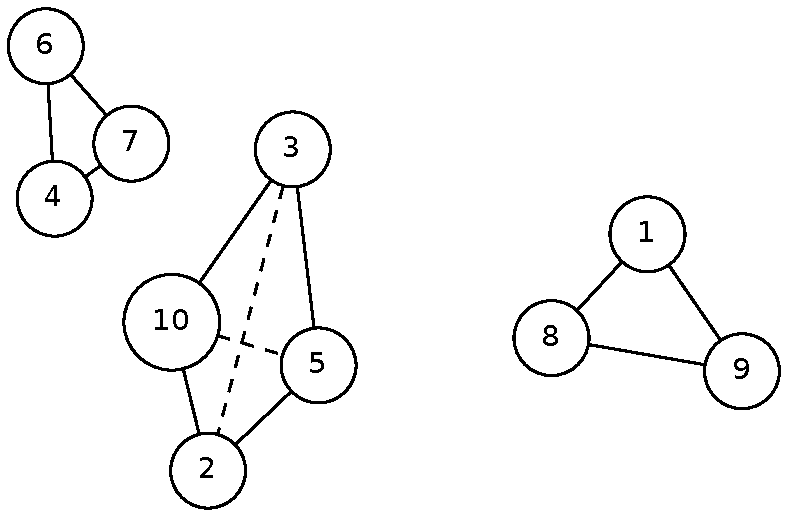
\includegraphics[width=0.8\linewidth]{figures/bendersa}
        \label{fig:sub1}
    \end{minipage}%
    \begin{minipage}{.1\textwidth}
        $\implies$
    \end{minipage}%
    \begin{minipage}{.45\textwidth}
        \centering
        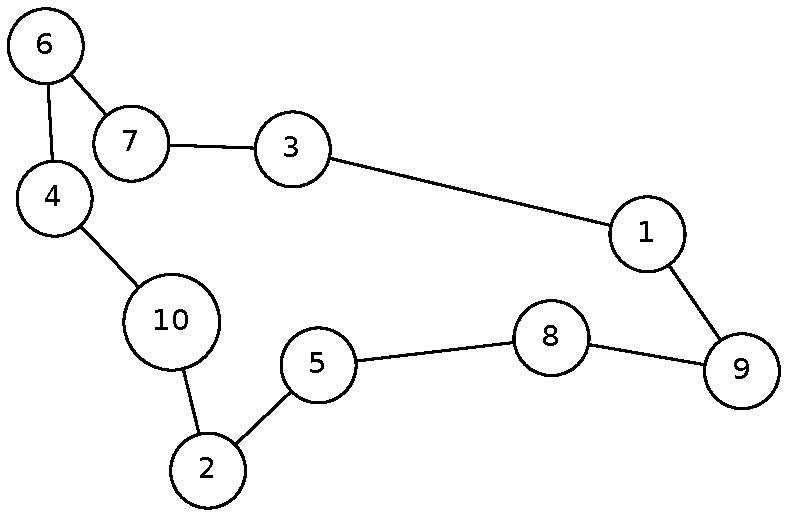
\includegraphics[width=0.8\linewidth]{figures/bendersb}
        \label{fig:sub2}
    \end{minipage}
    \caption[Benders example]{\centering Adding $x_{47} + x_{76} + x_{64} \le 2$, $x_{25} + x_{53} +
    x_{310} + x_{102} + x_{23} + x_{510} \le 3$ and $x_{89} + x_{91} + x_{18} \le
    2$ will prevent subtours to form, forcing a subtour-free solution}
\end{figure}

One thing that's important to keep in mind is that, during iterations, there's
no guarantee that the number of subtours is monotone nor decreasing. After some
iterations, let's say when such number are less than 5, we can have lots of
variability and the convergence to a single tour can be pretty slow. Also,
there's no thing such as subtours merging: adding two SEC doesn't mean that
those subtours will be merged in a single one, they can also form subtours in
other ways.

\subsection{Implementation details}
The last thing to specify are some details left behind. The MIP solver
that we will use is CPLEX. We can have more freedom in the connected component
algorithm, necessary for the creation of the constraints. We need both fast
insertion and fast retrieve the nodes of a component. This can be done adapting
a union-find data structure (with path compression and other heuristics) mixed
with a linked-list (implemented using swap ends trick). Notice that it's not
necessary to preserve the order of the subtour visit, we only need the nodes
that belongs to the same component. This could have been the best idea if the
number of subtours would be monotonically decreasing. Anyway, that idea works,
but it's a huge overkill, a simple successor vector (by sacrificing retrieve
time) or an adjacency list (specialized keeping 2 slots for node) can do the job
flawlessly. The second option is actual implemented, because it is reused in
future approaches to TSP. We have to state that the most of time will be spent
by the MIP solver, that will occupy the majority of the  available time limit.

\section{The Two-phase Loop method}
The time limit management for the Loop method is trivial: the MIP solver, for
the current iteration, can take advantage of the remaining time limit, that
will be split during each iteration. But, it's possible to notice, that after
some iteration the model became bigger and bigger (because of the SEC added)
and the MIP solver uses more and more time to solve the problem the single
subproblem. For this reason, considering an initial phase (phase 1) when we're
not interested in optimality, we can set a lower and fixed time limit for those
iterations, and so generate useful SEC to solve the problem. At the end of this
phase, even if we reach a single-tour solution, we cannot claim its optimality,
because we fixed our MIP solver to run constrained in time. We have then to let
run the solver indefinitely to reach an optimal solution (phase 2), as we did in
the usual Loop method. 

Since managing the time limit of CPLEX is too platform-dependent it's
possible to fix the maximum number of nodes generated or the maximum number of
incumbent updates: both of them behave like a time limit for phase 1's
iterations. The first strategy (setting \texttt{CPX\_PARAM\_NODELIM} in CPLEX)
is implemented.

We will refer this strategy as \emph{Two-phase Loop method}.

\begin{claim} 
    The improvement given by Two-phase Loop method is negligible.
\end{claim}

\begin{figure}[h]
    \centering
    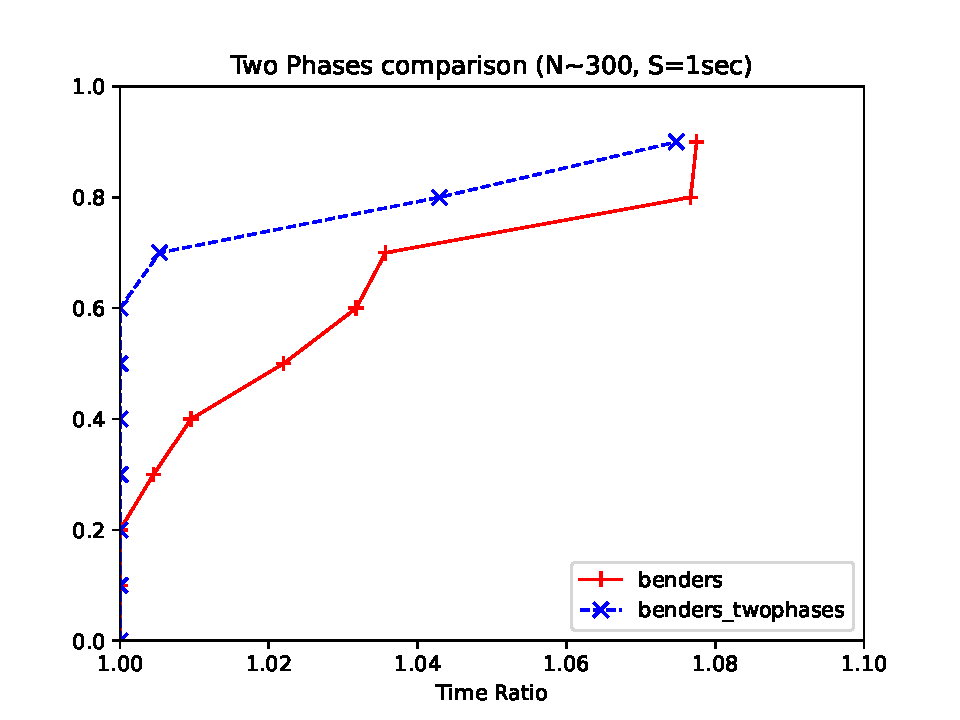
\includegraphics[width=0.8\textwidth]{figures/benders2phases}
    \caption{Loop methods comparison, short time ratio}
\end{figure}

Two hyperparameters have to be fixed, the amount of time spent on phase 1 and
the maximum number of branching nodes. We are not going to perfectly tune those
parameters, because performance variability will destroy our analysis, so,
after some tests on a validation set trying different parameters, we will fix
those to reasonable values: phase 1 will take 50\% of the time available,
during which only 3 nodes will be processed. More important details on
parameters tuning in appendix \ref{appendix:tuning}\\ The difference is
negligible, considering the very short time ratio, the two methods can be
considered equally valid.\\ Another reasonable strategy is to leave phase 2 the
shortest amount of time to solve to optimum the problem while using the
remaining time on phase 1. This strategy is better than the pure Loop method,
but the fifty-fifty split of time between phases seems the best.

\section{Callbacks method}
An adaptation of Benders method can be achieved using CPLEX's features:
\emph{callbacks}, a simple way to inject user-written code during
branch-and-cut. CPLEX uses branch-and-cut to solve MIP problems and, for each
node (excluding the special case of root node where some preprocessing also
happens), the fractional result obtained from LP relaxation is cut also using
cut pool's cuts to obtain an integer solution, then some primal
heuristics are applied to obtain a solution which will helpfully update the
incumbent. During these two phases (cuts application and before the incumbent
update) it's possible to generate and add constraints to the model using the
mechanism of callbacks. The idea behind this approach is that the user has more
insight than CPLEX about the problem, so it can add more specific and
problem-related cuts that will improve the computation.

This is different from Benders method, but the idea is similar: start
with SEC-free model, then adds, taking advantage of callbacks, all the SEC
necessary until a single-tour solution is obtained. We will refer to this method
as the \emph{Benders Callbacks method}.

The SEC added are, again, Danzing's SEC for symmetric version, but in two
different fashion. When adding a SEC before the incumbent update, it's possible to
recycle the connected components algorithm because an integer solution is
provided. The situation is different when trying to generate a SEC in the cut
callback because the code will be called back just after LP relaxation
solution, so just a fractional solution is available, and such a solution is a
mess, because we have some edges that are fixed to one and some other not, so
clearly not a collection of cycles. Anyway, an algorithm for finding connected
components given a fractional solution exists, and it relies on solving a
series of max-flow problems. Since the implementation is troubling, it's
possible to exploit a well-known library that will provide a subtour separation
procedure: \emph{Concorde}. The library's function for that task will be called
during the cut callback and some SEC will be added to the model. Those
constraints, as opposed to those generated before updating the incumbent, are
\emph{user
cuts}\footnote{\href{https://www.ibm.com/docs/en/cofz/12.8.0?topic=pools-what-are-user-cuts-lazy-constraints}{https://www.ibm.com/docs/en/cofz/12.8.0?topic=pools-what-are-user-cuts-lazy-constraints}}:
they are not needed to generate a feasible solution (single-tour) since we
already add all the useful SEC before the incumbent update, but they will help to
tight the model.

Let's now focus on the user cuts generation procedure. Considering the number of
nodes generated during branch-and-cut, the possible huge amount of SEC that are
possible to generate, the computing time required to generate those SEC, and the
fact that we're making our model bigger, one may ask if there this procedure
will add some overhead to CPLEX computation. The answer is positive: a model
with lots of SEC is great because it will tight the formulation, but considering
the amount of time spent generating those constraints and spent during
relaxations, it's necessary to find a trade-off. Some possible strategies are to
stop the generation of constraints if some requirements are reached. We're going
to present two strategies, by avoiding the separation randomly (per node) or
after a fixed number of nodes.
\newpage

\begin{claim}
    The Benders idea implemented through callbacks is superior to the Loop
    method. Stopping the constraint generation after a fixed number of nodes seems
    a good trade-off.
\end{claim}

\begin{figure}[h]
    \centering
    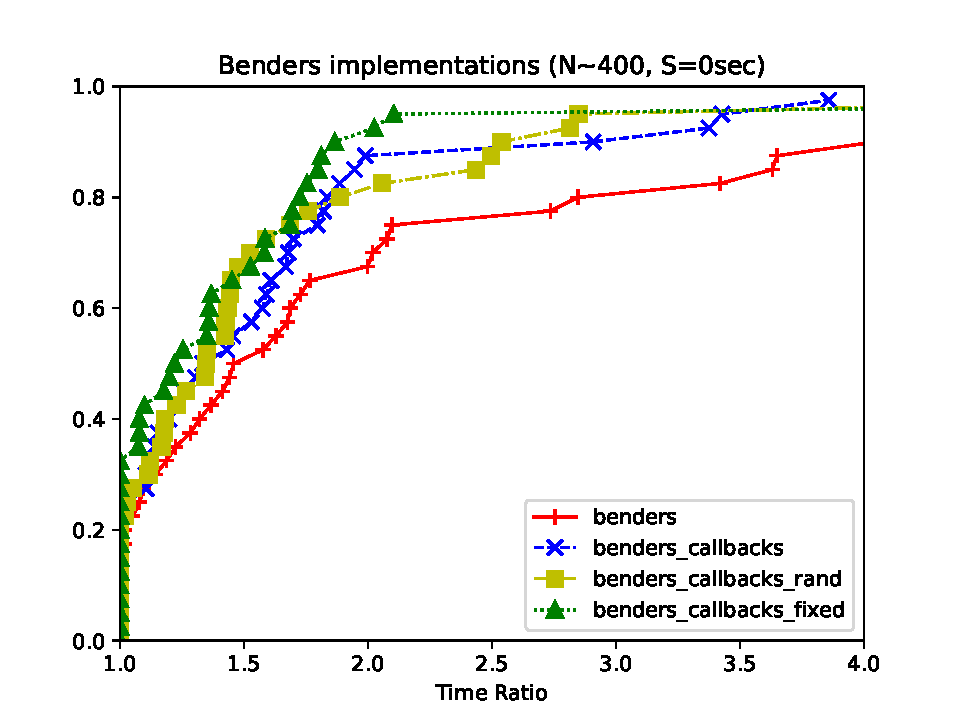
\includegraphics[width=0.8\textwidth]{figures/benders_final}
    \caption{Benders implementation comparison, with variants in callbacks}
\end{figure}

The comparison is done considering 40 instances of around 400 nodes each. Four
models have been compared: the Loop method and three variant of the callbacks
method: in one of them we stop the SEC generation (after LP relaxation) per node
randomly with 50\% probability, in another one, we stop after 64 nodes, and in
the third one we didn't stop the process at all, by adding as many constraints
as possible.\\
The hyperparameters we considered, 50\% and 64 nodes, are tuned using a
validation test, but not tuned to perfection considering performance
variability. Anyway, they both seem reasonable. Considering that with 400 nodes
per instance, the branching tree has usually $>10k$ nodes. The 50\% random
strategy simply cut by half all the possible SEC to be added. The fixed node
strategy is more like a bet: 64 nodes are way less than the total number of node
in the branching tree, we bet that the first explored nodes contain useful SEC to
be separated. 64 is chosen to be the first 5 levels in the branching tree,
considering a \emph{go-wide} strategy decided by CPLEX or the first 64 if CPLEX
decided to \emph{go-deep}. In this last case, we even bet on CPLEX's decision
ability.\\

The results show that the Loop method is inferior compared to the callbacks
method. The fixed nodes strategy seems slightly better than the other two, even
if the random strategy becomes competitive for a small slice of the time ratio. 
Anyway, both of them seem reasonable.


\chapter{Matheuristics}
\label{chap:Matheuristics}
An important category of algorithm to handle big instances is the family of
metaheuristics. In this section two matheuristics will be covered,
metaheuristics that uses mathematical programming. Heuristic techniques do not
aim to solve the problem to optimality but they look to find a good solution
close to it. The idea upon heuristics is a trade-off between precision and
performance. In fact, heuristics can handle way bigger instances than exact
models. We will explain the implementation of two different heuristics that
allow to solve instances that reach almost thousands nodes: Hard Fixing and
Soft Fixing. Both methods relies on the same idea. In two different ways the
aim is to find an initial feasible solutions and move to neighbours to getting
closer each step to optimal solution. To achieve this the two algorithms reduce
significantly the degree of freedom fixing a significant part of the solution. 

\section{Hard Fixing}
\emph{Hard fixing} technique was proposed in 1980 by Balas \cite{balas1980pivot} and
it is based on the simple idea to fix some variables to lower the dimension of
the problem to solve. In TSP it consists in fixing some arcs of the current
solution. The algorithm works as follows. An initial solution is found using a
MIP solver. Then, in every iteration, it is possible to fix some of the x
variables corresponding to the selected arcs by changing the lower bound to 1.
In this way arcs are forced to be selected again in the following iteration. At
the end of the iteration every arcs is freed setting the lower bound back to 0.


\begin{algorithm}[H]
\SetAlgoLined
\KwResult{An approximated solution}
    \emph{model} $\leftarrow$ Callback method model\;
    \emph{sol} $\leftarrow$ MIP non-opt sol (\emph{model})\;
    \While{timelimit not reached}{
        \ForEach{edge e in sol} {
            change $e$ lower bound to 1 with probability $p$
        }
        \emph{sol} $\leftarrow$ MIP opt (\emph{model})\;
        \ForEach{edge e in sol} {
            change $e$ lower bound to 0 with probability $p$
        }
    }
    \caption{Hard Fixing}
\end{algorithm}

It is important to notice that this new restriction to the problem does not cut
the current solution so in every iteration the solution will be at least as
good as before so the path of the objective function will be monotonically
decreasing.

\subsection{Implementation details}
The idea upon Hard Fixing is quite simple but, as often happens with
heuristics, it leaves many implementation choices. In our case the solution of
the MIP model is obtained as usual using CPLEX. At the very beginning of the
method the solution is found running the whole model on CPLEX allowing the
solver to run for a limited part of the timelimit with this portion that has to
be big enough to find a solution. A valid alternative can be to make CPLEX
solve the model only allowing to create the root node eventually leaving the
original timelimit. It can seem more convenient in terms of reliability but it
may stop the search for the starting solution too early. A good starting
solution is an important element to find a good approximation because in every
iteration the solution can move only to a close neighborhood. In our
implementation the starting solution runs for $\nicefrac{1}{10}$ of the total
timelimit. Then, the remaining timelimit is split between every iteration. In
our design the number of iteration is not set deterministically but each one
can run for $\nicefrac{1}{20}$ of the timilimit left from the first iteration. This
leads however to around 20-25 iterations\\ A further hyperparameter to tune is
the percentage of edges that have to be fixed at the beginning of each
iteration. This value can remain constant throughout the execution or variable
according to how much fast is the solution is moving. In our implementation we
decided to keep the most simple idea tuning this to 80\%.

\section{Soft Fixing}
A more recent work has been proposed in 2003 by Fischetti
\cite{fischetti2003local} is the \emph{local branching} also known as \emph{soft fixing}. The
aim is similar to the one in hard fixing trying to explore a neighborhood of
the current solution to improve iteration after iteration. While hard fixing
impose some edges to be selected soft fixing operates adding each time a
constraint to the model. The idea is to force the solver to find a solution
that changes at most $k$ edges. As before an initial solution has to be found by
the solver and every iteration has a certain timelimit to get an improved
solution. \\ To guarantee that the new solution is within a certain
neighborhood $k$ at every iteration the following constraint will be added \\
\begin{equation*} \begin{array}{rrlr} \displaystyle\sum_{(i,j) \in (x*)} x_{ij}
& \ge n-k \end{array} \end{equation*} imposing that at least n-k edges do not
change. In this way we ensure that the solution is contained

As before, this new constraint does not violate the current solution and CPLEX
automatically set it as the incumbent. This guarantee that when the solver hit
the iteration timelimit it return a solution at least good as before.
Furthermore, it is fundamental to remember that at every iteration before
adding the new constraint based on the new current solution it is necessary to
remove the constraint given by the previous solution.

While hard fixing has an intrinsic probabilistic approach selecting the edges
for a fixed $k$ the solution may not improve if is a local minimum. It surely may
happen in hard fixing too, but the hard fixing idea ensures that iteration
after iteration the solution space is explored differently. In soft fixing it
is useful if not necessary to define a policy to update $k$ when the solution
does not improve.

\begin{algorithm}[H]
\SetAlgoLined
\KwResult{An approximated solution}
    \emph{model} $\leftarrow$ Callback method model\;
    \emph{sol} $\leftarrow$ MIP non-opt sol (\emph{model})\;
    \While{timelimit not reached \emph{or} max k reached}{
        add the new constraint for k-neighborhood\;
        \emph{sol} $\leftarrow$ MIP opt (\emph{model})\;
        remove the constraint for k-neighborhood\;
        \eIf{sol not improve} {update k\;}{reset k to default}
    }
    \caption{Soft Fixing}
\end{algorithm}

\subsection{Implementation Details}
The steps are similar to hard fixing, so here we focus mostly on the policy of
updating $k$. Remember that $k$ is the maximum number of edges that can be changed
in a single iteration. The algorithm starts with $k$=3 and every time the
solution does not improve $k$ is increased by 2. Once the solution improve the
value is set back to the default value. If $k$ reaches 15 the algorithm
terminates. The starting iteration to find the first incumbent takes the 20\%
of the total time, twice of hard fixing one, because we expect that soft fixing
has a very good search among the neighborhood because its freedom among the
arch is bigger. However, for big instances hard fixing can change a lot of arch
in a single iteration, while soft fixing $k$ can be very small with respect to
the number of nodes.

A final remark, in the last iteration, both for soft and hard fixing, last
constraint has not to be removed because in this case CPLEX consider the
instance unsolved because it is modified after the solution is found.

\section{Matheuristics comparison}

\begin{claim}
    The hard fixing method is better on average instances, while soft fixing has better peaks when it start with a good solution
\end{claim}

\begin{figure}[h]
    \centering
        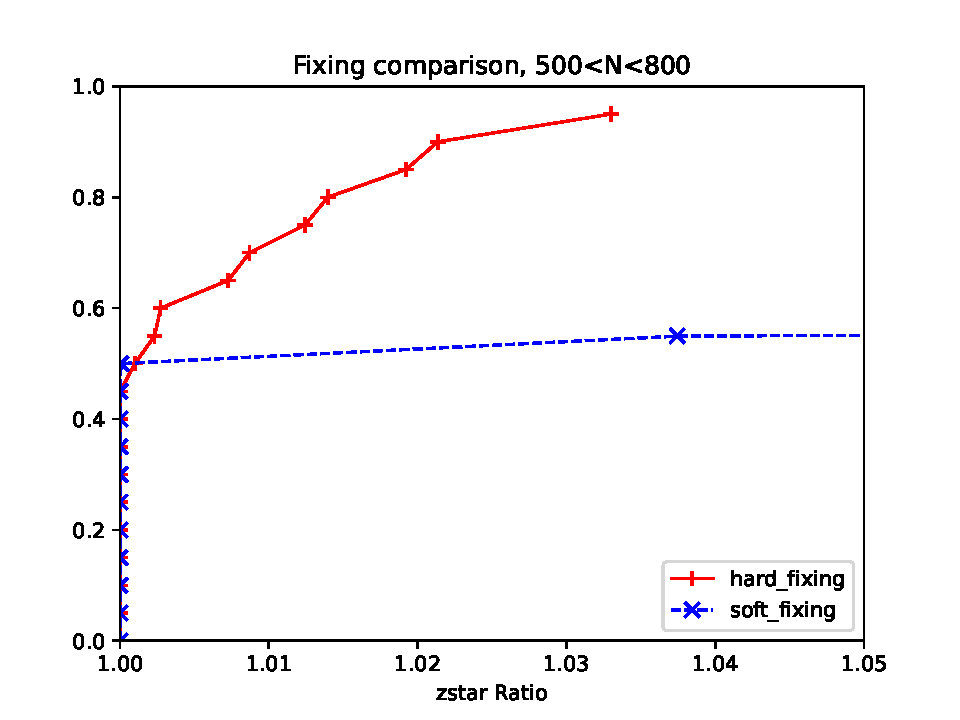
\includegraphics[width=0.8\linewidth]{figures/math}
        \caption{Matheuristics comparison}
\end{figure}

The comparison is done using random generated instances with a number of nodes
between 500 and 800 running for around 12 minutes each. The results showed that
hard fixing is quite consistent in returning a good solution even if it starts
with a bad one. In most of the cases it returns a solution within 2-3\% of the
optimum. Soft fixing, instead, strongly depends on the starting solution as we
expected. In fact, as stated before, in the hyperparameters tuning phase it
turned out that it was better to leave more time for the first iteration. It is
very clear observing the differences on how instances are solved. Almost every
time soft fixing find a good solution at the beginning it is better than hard
fixing and it comes very close to the optimal solution. As you can see they
split almost equally the victories but only once the loser solution of soft
fixing is close. Instead, all the times hard fixing is competitive. In fact,
when both start with a bad solution hard fixing manage to reach a good
approximation within the given timelimit, while for soft fixing is not the
case. When timelimit is too small it is a valid option starting with a k higher
than 3 because otherwise most of the iteration will lead to a very small change
consuming a significant part of the time.     


\chapter{Approximation algorithms}
In previous chapters, we dealt with methods that will produce an optimal
solution, if we provide them enough execution time. The challenge is to solve
problems with a huge amount of nodes, and for that reason, we have to drop
optimality seeking different strategies. But if we still have a feeling for
optimality, the choice is to move to approximation algorithms.

In an approximation algorithm, it is theoretical-guaranteed that the solution
is less then a factor $k$ from the optimal (since we're dealing with a
minimization problem), but the algorithm could also return a better one (even
the optimal one!).

The algorithms we're going to present works for a restricted version of the
problem: $\Delta$-TSP, in which the costs follow triangular inequality ($c_{ij}
\le c_{ik} + c_{kj},\ \forall\ i,j,k$). Since euclidean distance respect those
rule, Euclidean TSP is a restricted version of $\Delta$-TSP.

\section{$2$-approximation algorithm}
A $2$-approximation algorithm follows a simple idea: the optimal tour without an
edge, in a graph-theory point of view, is a single path visiting all the nodes.
Since that path is connected and acyclic, the path represents a spanning tree of
the nodes, which cost is greater than the shortest spanning tree (because that's
the shortest one) and less than the optimal tour (since we removed an edge).

\begin{equation*}
    cost(SST) \leq cost(path) \leq cost(optimal\ tour)
\end{equation*}

Let's now build a tour starting from the SST and doubling its edges by creating
a direct version of the tour. From that we will create a tour visiting each node
only once (a Hamiltonian cycle) by \emph{short-cutting} operation: starting
from the root node and standing on a node $a$, we will add the arc $(a,b)$ where
b is the next, unvisited node of the tour starting from $a$ or the root node if
there's no remaining node to visit. 

\begin{equation*}
    cost(tour) \leq 2 \cdot cost(SST) \leq 2 \cdot cost(optimal\ tour)
\end{equation*}

For this reason, we can talk about \emph{$2$-approximation algorithm}.

\begin{figure}[h]
    \centering
    \begin{minipage}{.3\textwidth}
        \centering
        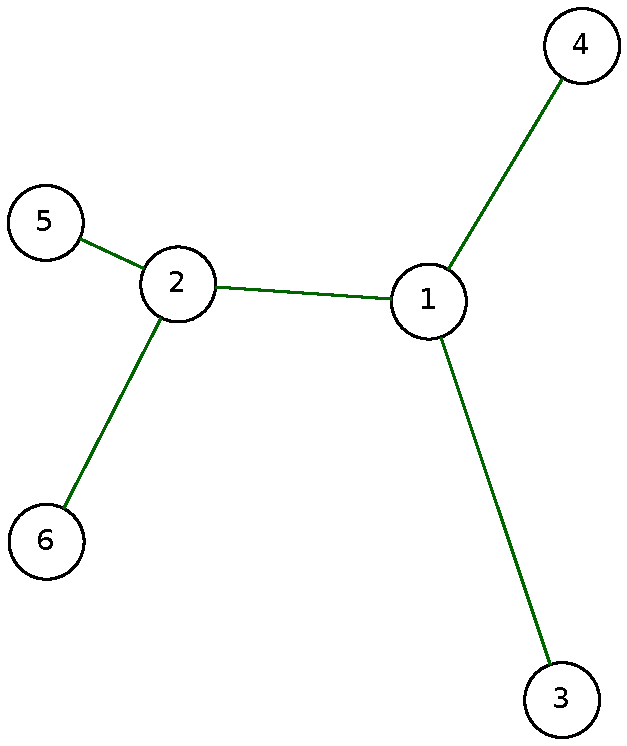
\includegraphics[width=0.8\linewidth]{figures/2approxa}
        \label{fig:sub1}
    \end{minipage}%
    \begin{minipage}{.3\textwidth}
        \centering
        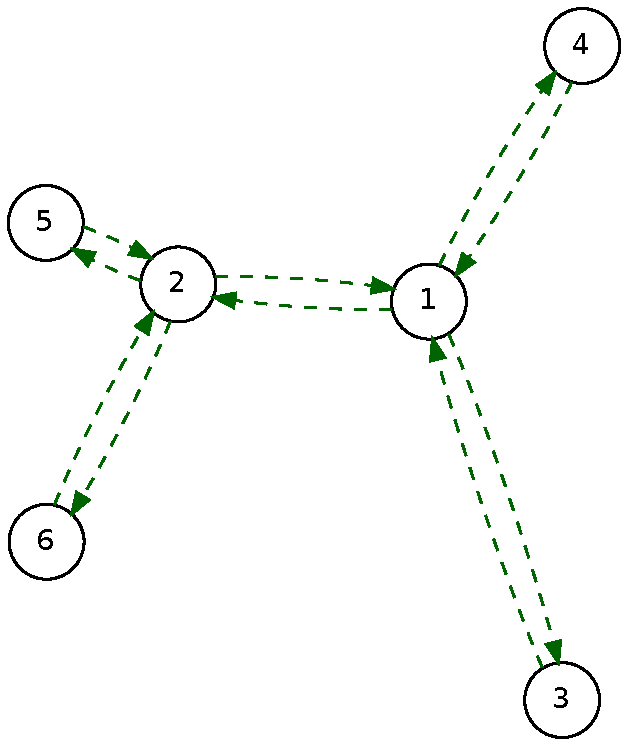
\includegraphics[width=0.8\linewidth]{figures/2approxb}
        \label{fig:sub2}
    \end{minipage}
    \begin{minipage}{.3\textwidth}
        \centering
        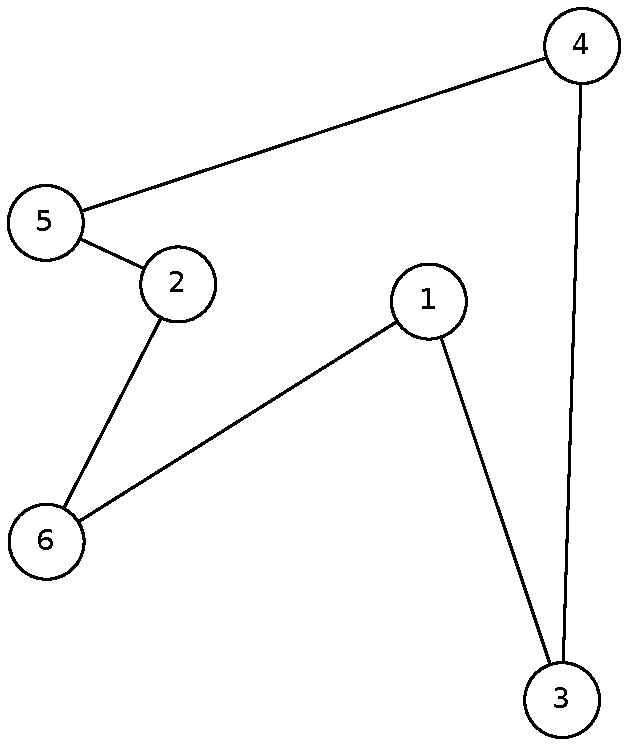
\includegraphics[width=0.8\linewidth]{figures/2approxc}
        \label{fig:sub2}
    \end{minipage}
    \caption[Shortcut example]{\centering Starting from 5 (root), the post-order visit of the tree
    is: 5 2 6 (2 skipped) 1 3 4 5}
\end{figure}

\subsection{Implementation details}
Kruskal's algorithm is implemented for the SST. Internally, it uses a
path-compressed union-find data structure mixed with classical node pointer
implementation of a tree. An additional data structure is implemented for the
visit because the union-find (especially when path compressed) doesn't track the
tree structure. In this way, both the SST computation and visit are fast
($\mathcal{O}(|V|^2log|V) + \mathcal{O}(n)$).
For this algorithm, some degree of freedom is available to tune: since an
undirected tree has no root, one may choose the node he prefers. The visit also
can be adapted, a post-order visit that starts from the union-find root has been
implemented for convenience, but a pre-order also works fine. To be honest, the
most trivial way is to topologically visit the tree starting from node 1. Both
approaches are equivalent since the theoretical guarantee is respected.
The approach is not optimal for the $\Delta$-TSP problem: some crossing may
pop out. Dealing with this kind of situation will be discussed subsequently.

Since its direct competitors will be introduced in
\autoref{chap:metaheuristics}, we're going to present results later on.

\section{$\nicefrac{3}{2}$-approximation algorithm}
A $\nicefrac{3}{2}$-approximation algorithm has been developed by Christofides,
a British mathematician in 1976. It was the best approximation algorithm for
many years, and its main idea is very similar to the one we just presented but
with a twist: the author thought that doubling the edges of the SST was too
expensive: instead of that, one could simply add some edges to the tree until an
\emph{Euler cycle} (a tour that touches each edges exactly one) has been formed.
This Euler cycle touches some nodes multiple times, and it needs to be
shortcutted to obtain a Hamiltonian cycle. The extra edges can be found
using a \emph{matching} of the graph (set of edges without common nodes) that
can be computed in polynomial time (even if $\mathcal{O}(n^3)$).

Since this algorithm is not good in practice (even considering the
theoretical guarantee), it will not be implemented.


\chapter{Heuristics}
\label{chap:Heuristics}
Let's suppose now we have no feeling at all for theoretical optimality
guarantees, we just want to obtain a solution as fast as possible and,
hopefully, a good one. That's when the \emph{heuristic} approaches take place:
they're fast algorithms (typically polynomial) and in some cases, on average,
they're close to the optimal solution for no more than 2-3\%. Again, there's no
theoretical guarantee on the worse case, but in practice they work pretty well.

We can split heuristic approaches into two subcategories:
\begin{itemize}
    \item \emph{Constructive heuristics}: they built a solution from scratch
    \item \emph{Refinement heuristics}: starts with a solution while iteratively
        improving it. Hard and Soft Fixing are examples of this category
\end{itemize}

\section{Constructive Heuristics}

\subsection{Greedy}
The first constructive heuristic we're going to present follows a \emph{greedy}
strategy to solve TSP: sitting in a node, the next one in the path will be the
one at the shortest distance or, if there are no other nodes to visit, the tour
returns to the starting node. The approach follows the greedy paradigm
because at each node it selects the best local solution, i.e., the closest
node.\\
Excluding the starting node and the last one (that closes the loop), we have to
repeat the process $n -2$ times (let's say $\mathcal{O}(n)$) in which we have to
select the next node among $\mathcal{O}(n)$ possibilities. The algorithm runs in
$\mathcal{O}(n^2)$, which is pretty fast compared to a MIP solver. For that
reason, it's possible to repeat the greedy process for each node and finally
select the best tour among all solutions by raising the computational complexity 
to $\mathcal{O}(n^3)$, which remains fast enough.\\

An important thing to notice is that the algorithm is fully  deterministic,
there's no room for parameter tuning or different strategies. If one would
impose a time limit on this method, it could simply stop the computation and
keep the best solution found until the stop.

\subsection{GRASP}
To spice things up, one could extend the greedy paradigm by injecting randomness
into the process. One possibility is to randomize the greedy choice among the best
$k$ options one may have while selecting the next node. This introduces
variability and, in the long run, this approach produces better results. Another
thing that is possible to randomize is the initial choice of the starting
node. We will refer to this as \emph{GRASP: Greedy randomized adaptive search procedure}\\
The approach runs in $\mathcal{O}(n^2)$ for starts, but since the randomness in
the tour and the randomness of the starting node, this approach could run
indefinitely. It will search among a subset of the (finite) possible subtours
according to the greedy choice. For this reason, this approach will run until a
time limit is reached.

\subsubsection{Implementation details}
The greedy approach implementation is straightforward.\\ 
For the grasp approach, a data structure that maintains the top-$k$ choices is
implemented as a priority queue that is implemented as a max binary heap of
fixed $k$ elements. Notice that, even if we're searching for the
shortest-distances node (so we have to minimize the distances in our data
structure), we're only interested in fast retrieval of the distance of the
$k$-th node. In this way, one could pop out that node if a shorter distance
node is encountered. Then, one of the $k$ nodes in the pool can be randomly
chosen.

\subsection{Extra Mileage}
Another constructive heuristic is based on a simple move that builds a solution
starting from a subtour. Suppose that we want to add node $x$ to the tour,
ideally, we're going to break the closest edge $\{a, b\}$ to that node and add
two new edges, $\{a, x\}$ and $\{x, b\}$ so the new node is included. This is
called \emph{extra mileage move}, because among all the possible edges already
included in the tour and all the nodes not included (suppose that we want to
search also the best $x$) it's ideal to perform a move on the ones that
minimize the \emph{extra mileage} $\Delta_{\{a,b\},x} = c(a,x) + c(x, b) - c(a,
b)$. We will repeat this move until a tour has been formed.

\begin{figure}[h]
    \centering
    \begin{minipage}{.33\textwidth}
        \centering
        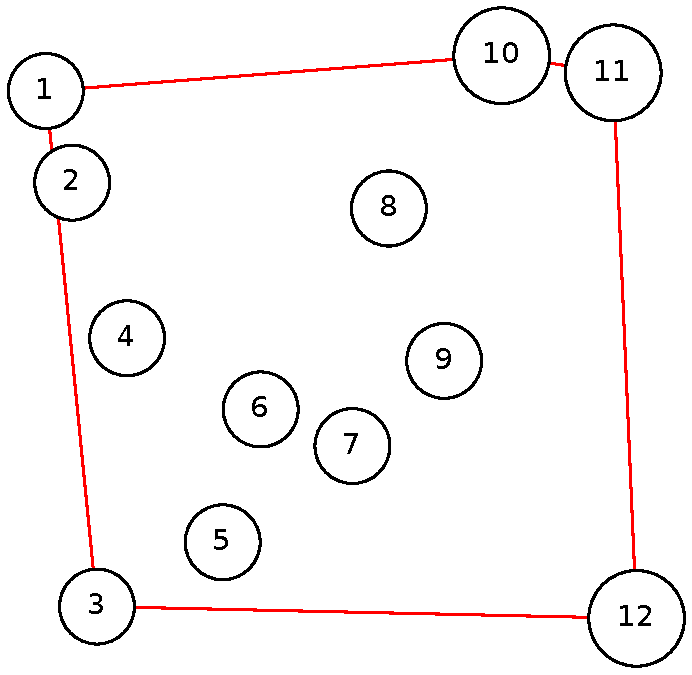
\includegraphics[width=0.8\linewidth]{figures/heura}
        \label{fig:sub1}
    \end{minipage}%
    \begin{minipage}{.33\textwidth}
        \centering
        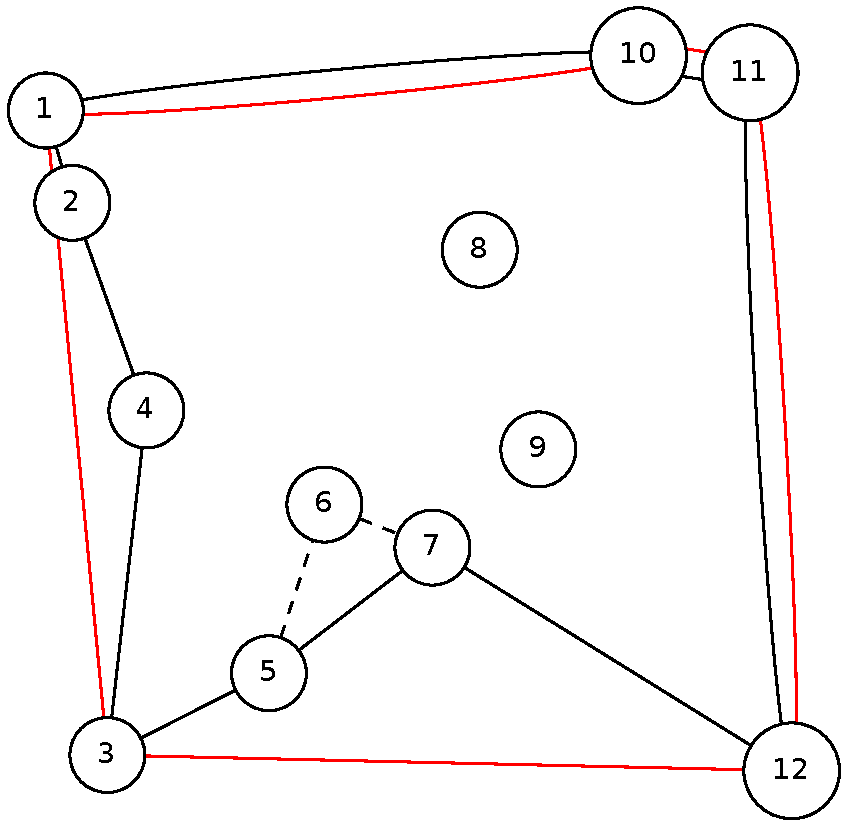
\includegraphics[width=0.8\linewidth]{figures/heurb}
        \label{fig:sub2}
    \end{minipage}
    \begin{minipage}{.33\textwidth}
        \centering
        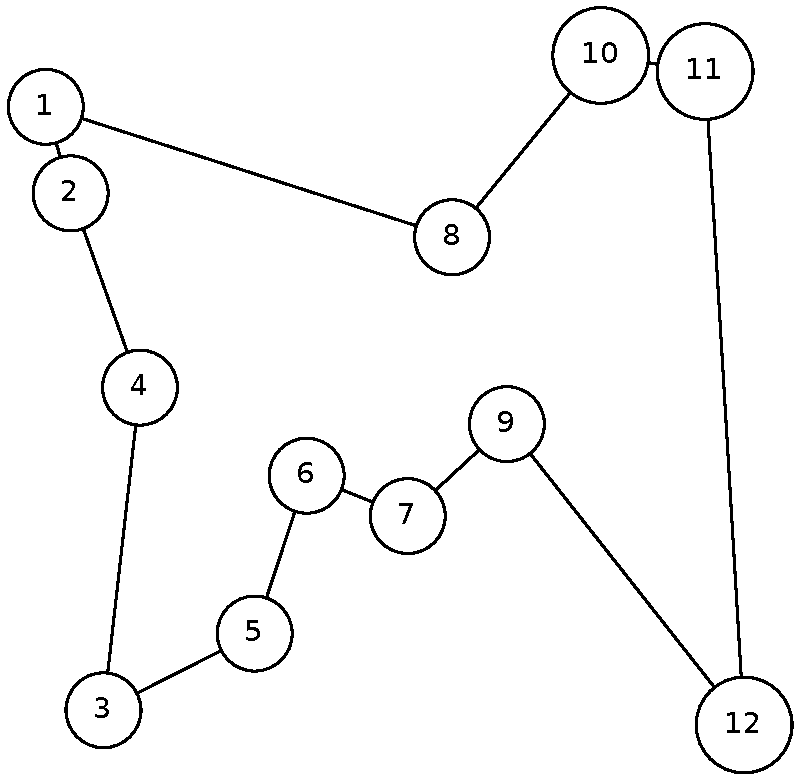
\includegraphics[width=0.8\linewidth]{figures/heurc}
        \label{fig:sub2}
    \end{minipage}
    \caption{\centering Extra mileage algorithm starting from convex hull}
\end{figure}

Since selecting an edge and a node that minimizes the extra mileage will take
$\mathcal{O}(n^2)$, and since we have $\mathcal{O}(n)$ nodes to include in the
tour, the algorithm runs in $\mathcal{O}(n^3)$. The algorithm, as greedy, is
fully deterministic.\\
There's multiple ways to select an initial subtour, in principle, any could work.
Anyway, there are two preferred choices: starts from a subtour of the two most
distant nodes or starts from the frontier of the convex hull, the unique and
smallest set that encloses all the nodes.

\subsubsection{Implementation details}
The implementation is straightforward. It has been selected to start from the
convex hull of the nodes, computed with a popular Graham's scan variant:
Andrew's Monotone chain algorithm, bases on counter-clockwise turn substructure
property that runs on $\mathcal{O}(nlogn)$, anyway absorbed in the
$\mathcal{O}(n^3)$ total complexity.

\subsection{Constructive heuristics comparison}

\begin{claim}
    Extra milage and greedy are good algorithms, leaving aside the computational
    cost. GRASP have the same performance as greedy. 2-approx, despite the
    guarantees, is not a good algorithm.
\end{claim}

\begin{figure}[h]
    \centering
    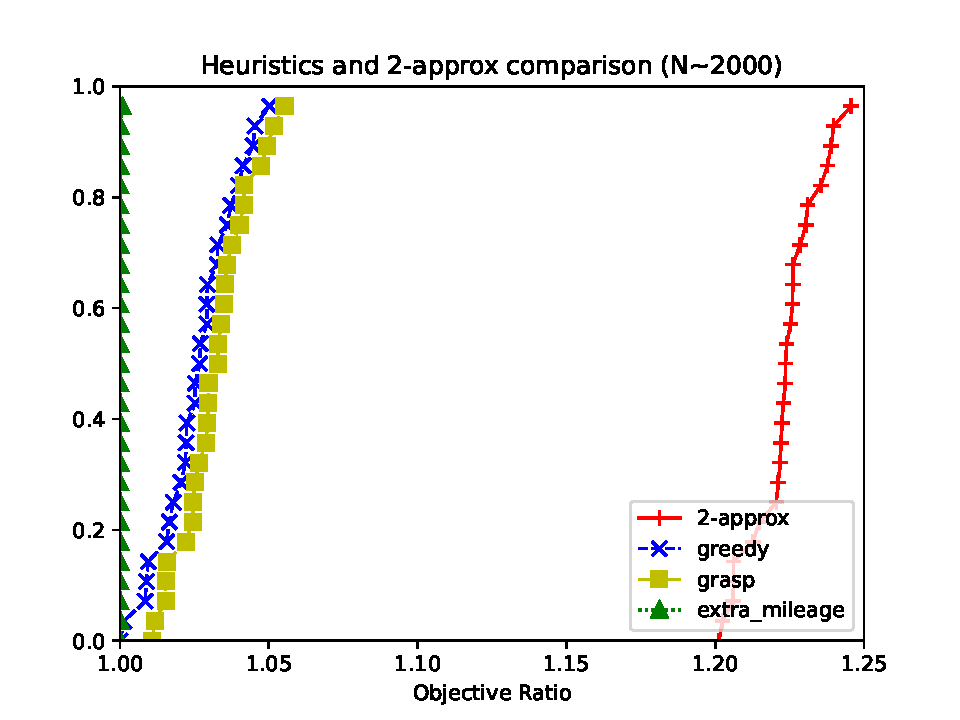
\includegraphics[width=0.8\textwidth]{figures/heuristic_firstcomp}
    \caption{heuristics and 2-approx comparison}
\end{figure}

A first comparison has been done on 30 instances of 2000 nodes each. The graph
presented has the same meaning as the previous ones, except that
the objective function is considered instead of times. The number of nodes has
been chosen to let the $\mathcal{O}(n^3)$ algorithms run in a reasonable amount
of time by letting them reach convergence. \\
The winner is Extra Mileage algorithm, which has the same
complexity as greedy, both achieves good results. The main difference between
these approaches is that greedy's results are the best results among various
runs of the algorithm (by considering different starting nodes) while extra
mileage just produces one result. This can be a huge disadvantage considering
that it's not possible to set a time limit at all: while greedy even if stopped
will produce some good results, extra mileage will not, and time limit
management will be crucial in future approaches. \\
GRASP can be considered as good as greedy, even more flexible because of
randomness. In this test, grasp seems to achieve worse results compared with
greedy and this can be due caused by two factors: a sub-optimal tuning of $k$
(set to $5$) and especially the time limit management. Even if we compared
different algorithms with different behaviors, a common time limit has been
chosen to let the $\mathcal{O}(n^3)$ converge (especially extra-mileage
that will produce only one result). In this settings, also greedy will converge
and that means that the algorithm has explored all possible starting nodes, but
that will not happen with bigger instances, when even if let run for a
reasonable amount of time, the algorithm will explore only a small subset of all
possible starting nodes. And that's when grasp's randomness will become
competitive.\\ 
Recalling that it belongs in a different category, 2-approx's performances are not
exciting, even it's very fast: it produces just one result as extra mileage, and
it's not tunable at all. There's no room for improvement.

\section{Refinement heuristics}

Even without theoretical guarantees, a heuristic is considered decent if it
reaches 5\% from optimality, while the most sophisticated ones  can reach <1\%.
The constructive heuristics we presented, unfortunately, will not easily reach
those results: they will need refinement. \\
Refinement heuristics, applied to an initial yet feasible solution, will improve
the results by exploiting a simple property of euclidean distance.

\subsection{$k$-opt moves}

In $\Delta$-TSP (but also in Euclidean TSP since it's a particular case) the
costs must respect with triangular inequality $c_{ij} \leq c_{ik} + c_{kj},\
\forall\ i, j, k$. By keeping in mind this  property and since we're mainly
working in the case where nodes are 2D coordinates-located cities, a solution
can be improved if a \emph{crossing} is detected. The reason is that, by
triangular inequality applied to the triangle that forms with the center of
the crossing, it's always possible to reach the city $c$ from $a$ directly instead
of reaching it by moving first into another one $b$ and then follow
that leads to $c$.\\
This crossing-deletion procedure is the main idea behind \emph{$k$-moves}:
when a crossing is detected it is deleted, and instead of it two new arcs will be
added. This particular case where the arcs involved are two is called $2$-move.
It's possible to generalize to $k$-move: a rearrangement of $k$ arcs in a way to
reduce the cost of the solution.\\

Considering $x^H$ the current solution, $k$-opt moves can be interpreted in another
way. A move defines a translation of $x^H_0$ in the solution space within a
neighborhood as large as $k$ improves. By rearranging a huge amount of arcs,
there's a lot of room for improvement and so the neighborhood is larger. This is
the same interpretation as we did in Chapter \ref{chap:Matheuristics}. After
a move has  been applied, the new current solution $x^H_1$ is centered is
another neighborhood and the process is repeated until the solution cannot be
improved no more, stuck in a \emph{local optima}. The entire process can be
repeated considering another fresh new solution $x^H_0$. We will refer to this
as \emph{multi-start}, that can be repeated until a time limit is reached.

\subsubsection{$2$-opt moves}
Let's focus on $2$-opt moves. We're still considering the symmetric formulation of
the problem, but let's move to the asymmetric one for simplicity (that's why
before we talked about arcs and not edges). Suppose we found a crossing between
arcs $a \rightarrow b$ and $c \rightarrow d$. The move can be summarized in this
way: remove the arcs $a \rightarrow b$ and $c \rightarrow d$, add $a \rightarrow
c$ and $b \rightarrow d$, and, because the solution has to remain feasible,
reverse the path $b \leadsto c$.

\begin{figure}[h]
    \centering
    \begin{minipage}{.45\textwidth}
        \centering
        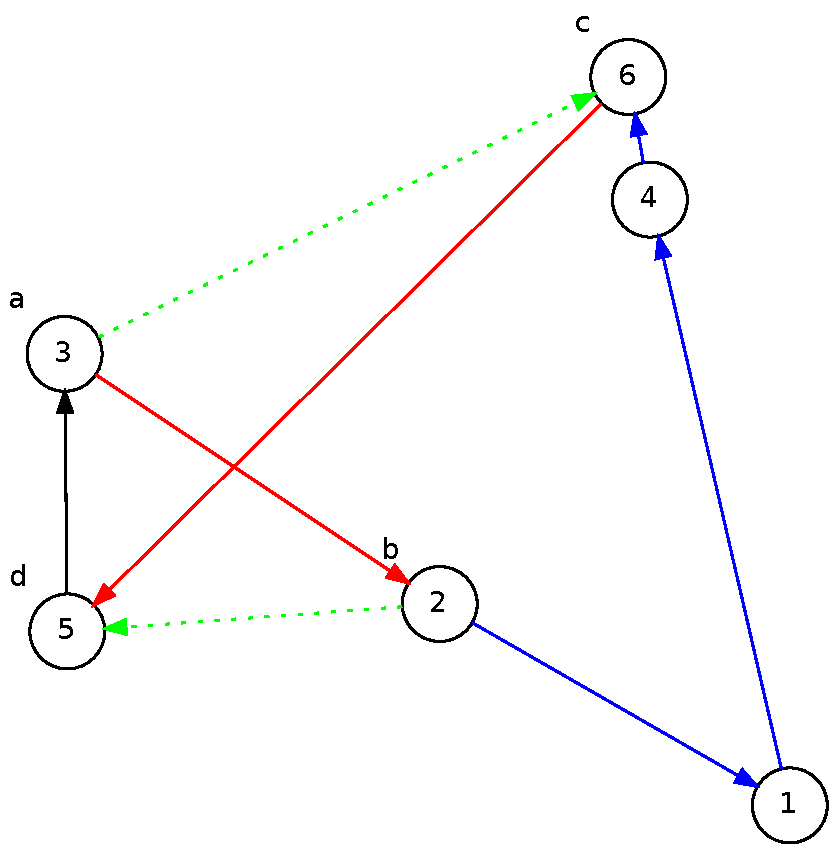
\includegraphics[width=0.8\linewidth]{figures/2move_before.pdf}
    \end{minipage}%
    \begin{minipage}{.45\textwidth}
        \centering
        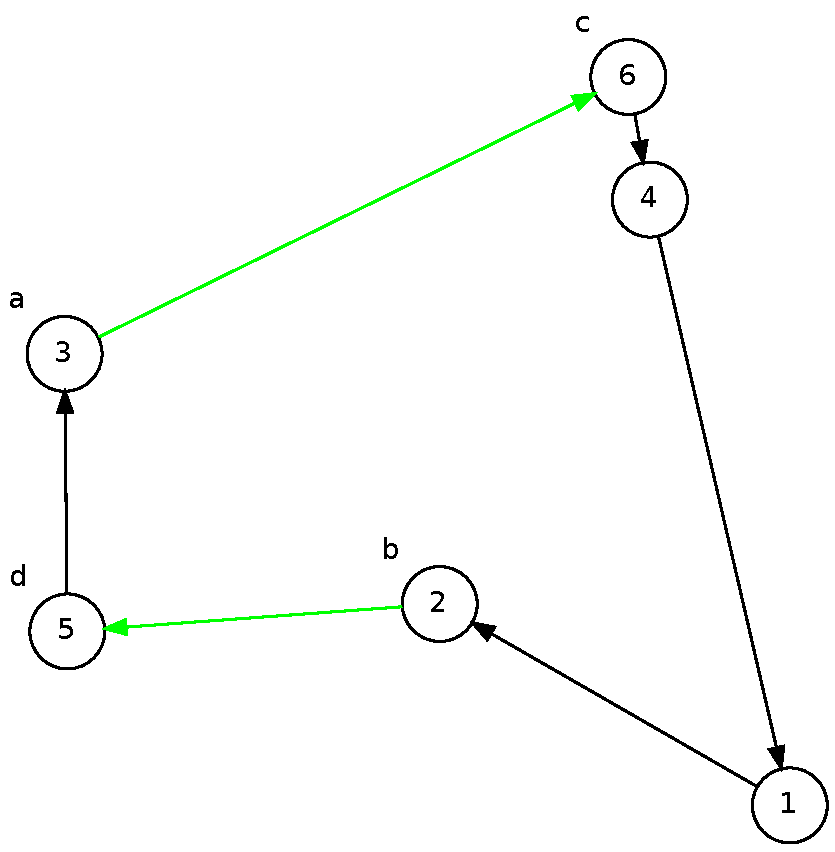
\includegraphics[width=0.8\linewidth]{figures/2move_after.pdf}
    \end{minipage}
    \caption[$2$-opt move example]{\centering $2$-opt move example: red arcs needs to be deleted, green
    to be added and there's the blue path to reverse}
\end{figure}

While it's possible to reverse a huge number of arcs ($\mathcal{O}(n)$), it's in
practice a very fast operation.\\
The last thing to do is a crossing-detection algorithm. There exists a
computational geometry sliding window-based algorithm, but since we're working
with costs it's possible to detect a crossing by analyzing the following value:

\begin{equation}
    \Delta(a,c) = c_{a,c} + c_{b,d} - [c_{a,b} + c_{c,d}]
\end{equation}

This corresponds to the difference between the objective function of the new
tour minus the old one, after a move that involves nodes $a$ and $c$. Notice
that even if we're working on the asymmetric formulation since we started from
a symmetric one, the reversed path has the same cost as the original one, and it
does not matters in the formula. If $\Delta < 0$ there's a crossing and a $2$-move can
be applied.\\
Among all the possible moves that can be applied to a solution $x^H_k$, one
may choose the one with minimum delta or just the first one that encounters.
Since a move is applied starting from a pair of nodes (and their successors),
one may possible to search among $\mathcal{O}(n^2)$ possible moves to find the
one with minimum delta, which sounds fair because the computation of $\Delta$
and the move are cheap operations.

\subsubsection{$3$-opt moves}
After a solution has been refined with all possible $2$-opt moves it becames
crossing-free, but there's still room for improvement. One thing that is
possible to do is to enlarge the neighborhood size by considering $3$-opt moves to
search for better solutions.  Now the thing starts to become complicated
because, to search for minimum $\Delta$, we have to search among
$\mathcal{O}(n^3)$ triplets of nodes and as opposed to previous case, among a
single triplets there's multiple way to reconnect the arcs, and so multiple way
to compute $\Delta$. Both searching and reconnecting are more costly.\\ 
For this reason, usually, this kind of refinement heuristics are implemented so
multiple cheap operations are preferred to few, costly, ones. And so $2$-opt moves
and $3$-opt moves are preferred over $k$-opt moves with $k$ elevated, since it will run
in $\mathcal{O}(n^k)$

\subsection{Implementation details}
Multi-start refinements with moves lead to lots of possibilities in terms of
tuning, that take shape in form of time limit management. The first, obvious,
thing to test is how far we can move in term of neighborhood size. In case of
$3$-opt moves, after the generation of a starting solution (using GRASP), we're
going to apply as many moves as possible, followed by as many $2$-opt moves as
possible. If we want to restrict on $2$-opt moves only, we can clearly skip the
application of $3$-opt moves. If during one of this processes the computation
reaches time limit, the computation for that start is stopped and the best
solution among all starts (also considering the actual partial one) is
returned.\\ One thing that one could may ask is if is more clever to allow more
starts (and so keeping the computation light, maybe skipping $3$-opt moves) or
bet on few, more optimized but heavy, computations.

\begin{claim}
    Skipping $3$-opt moves and allowing more starts is a good idea.
\end{claim}

\begin{figure}[h!]
    \centering
    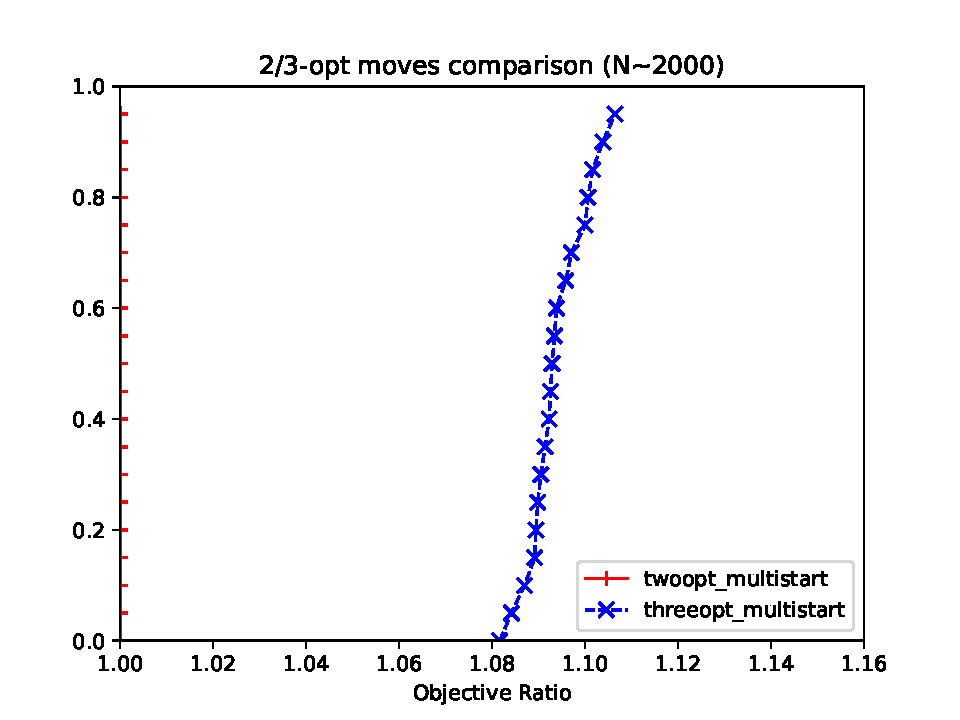
\includegraphics[width=0.7\textwidth]{figures/twothree}
    \caption{Comparison between $2$-opt and $3$-opt moves multi start}
\end{figure}

Our tests on 20 instances of 2000 nodes each shows (even if it's difficult to
visualize) that skipping $3$-opt moves is a good idea. In practice, in the
majority of executions, while with $2$-opt moves only there's multiple restarts,
that allows to pick a good solution, the computat stops before all the
possible $3$-opt moves can be found and applied, so it stuck on the first start.
Actually only few of them are applied and, even if the objective improves a lot,
this approach is worse than apply lots of small improvement.\\

Let's now focus on the initial solution generation. As stated before, GRASP is
used for the process, but one could choose to let internally run GRASP for a
greater amount of time in order to obtain a better inintial solution, that means
few crossing to fix and more multiple starts to perform in the same time limit.
Is it worth spending more initial time on GRASP?

\begin{claim}
    A better initial solution is preferred in multi start approach.
\end{claim}

\begin{figure}[h]
    \centering
    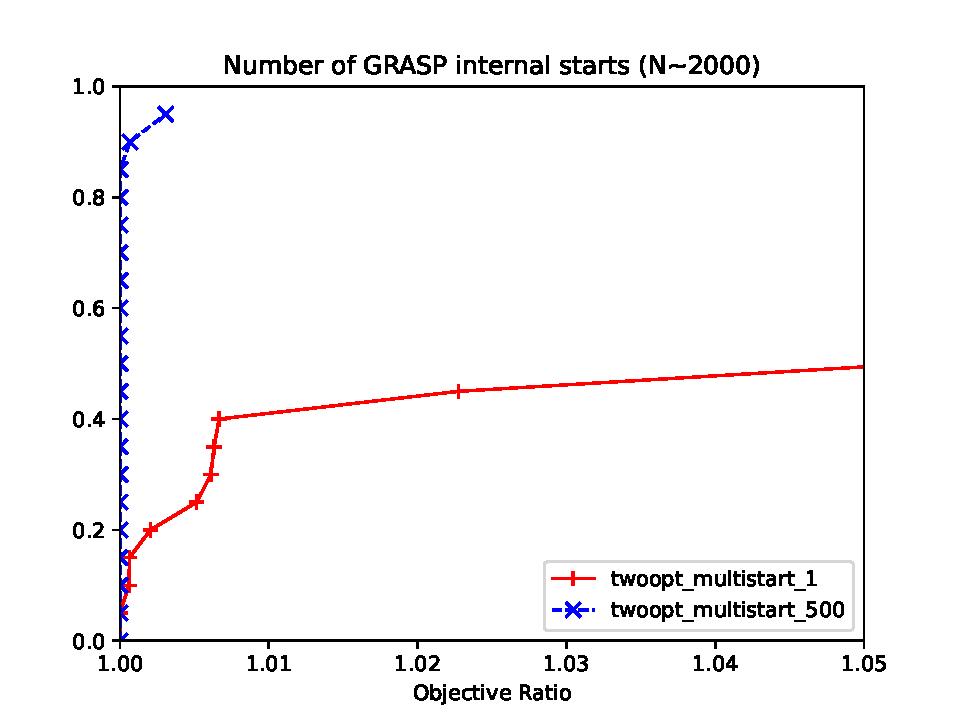
\includegraphics[width=0.8\textwidth]{figures/grasp_starts.pdf}
    \caption{$2$-opt moves multistarts on different GRASP internal starts}
\end{figure}

We tested 20 instances of 2000 nodes each, where the comparison is between
$2$-opt moves refinements considering two scenario for the initial starting
solution $x^H_0$: the first one found by GRASP and the best among 500 starts of
the constructive heuristic, a huge amount considering that is $\nicefrac{1}{4}$
of the total number of nodes. The initial computational cost is clearly higher
but, since it's a better solution, it presents fewer number of crosses and so
the $2$-opt refinement will take less time, (since it's the most costly
operation within a start). The best objective improves, as it can be seen in the
graph, for a single start (because it starts from a better solution) and in
general because, with the time saved, more starts are possible, which doubles.
Since we notices a bit of variability of refined solutions in different starts,
this can only be beneficial.


\chapter{Metaheuristics}
\label{chap:metaheuristics}
The last category of approaches to solve TSP are \emph{Metaheuristics} we're
going to present, high-level and complex procedures that are powerful enough to
reach near-optimum solutions in a reasonable amount of time, even with huge
instances. Considering the NP-hardness of TSP, this is our best shot so far, if
we're satisfied with an approximate solution. Internally they uses the
precedent heuristics we presented: they're placed at the implementation level
considering the high-level formulation of metaheuristics.\\ Among all the
approaches presented during the years, we're going to introduce three of them that
works nicely on TSP.

\section{Variable Neighborhood Search}
\emph{Variable Neighborhood Search} (VNS) is a metaheuristic technique proposed in
1997 \citep{mladenovic1997variable}. When an algorithm explores a solution space
not using mathematical programming the final result may be very influenced by
the starting solution. Sometimes allowing the algorithm only to improve the
solution can stuck it in local minimum that can be way worse than the optimal
solution. So VNS consents the current solution to move in a random way to
give it a chance to escape from these points of minimum.\\

\begin{algorithm}[H]
\SetAlgoLined
\KwResult{An approximated solution}
    $x\ \leftarrow$ initial solution\;
    \While{time limit is not reached \emph{or} $k \le k_{max}$}{
        $x'\ \leftarrow\ shake(x, k)$\;
	    $x' \leftarrow\ localopt(x')$\;
        \eIf{$cost(x') \le cost(x)$}{$x \leftarrow x'$\;}{$k \leftarrow k+1$\;}
    }
    \caption{VNS}
\end{algorithm}

So, the procedure of VNS needs two fundamental element: the method that
improves the solution and the one that can disturb it to escape from possible
local minimum. The \emph{shaking} function that disturbs the solution usually
depends on a input value $k$ that defines the neighborhood size Then the local
search function finds a local minimum. If this new solution is better then the
one before it becomes the incumbent, otherwise the neighborhood size increases
by one. If the max neighborhood size is reached the algorithm stops.

\subsection{Implementation details}
In our implementation of VNS we adapt the possibility to start from a random
solution or from a precomputed one. More on this choice in the next section,
since we're going to face similar choices. In TSP terms the shake operation is
called \emph{kick}, as it is slightly modifies the incumbent by rearranging $k$
arcs. The procedure clearly has to modify the solution into a feasible on, the
implemented procedure has to be subtour-free. The new candidate solution is then
modified using $2$-opt moves refinement presented is the previous chapter since,
as claimed, for an interesting number of nodes, there's no point of using
$k$-opt moves, with $k \ge 3$.\\ 
Every time a better solution is found the incumbent is updated and VNS is reset
with starting $k$ value equals to some minimum, 3 in our implementation. In the
case that the local search did not produce a new optimum the neighborhood is
enlarged by increasing $k$, until $k$ reaches $k_{max}$, where the algorithms
terminates. The increment of $k$ as well as $k_{max}$ should be tuned according
to the time limit, since it's not optimal to waste time on small $k$ with no
improvements or waste possibilities by truncating the computation due to small
$k_{max}$.\\
This can be seen as a multi-start procedure as the one presented above, but with
a kicked solution instead of a total different one.


\section{Tabu Search}
\emph{Tabu Search}, among with VNS, is another important metaheuristic proposed
by Fred Glover in 1986\citep{glover1986future} and, as VNS, is based on
refinements.\\ Starting from a solution, one is willing to improve it with
refinements until a local optimum is reached (\emph{downhill}). From there, one
could restart from another initial solution (multi-start) or restart from a
similar one by shaking it. Instead of those solutions, it's possible to insist
on the refinement subroutine and apply the refinement anyway. Since the solution
is stuck in a local optimum, the refinement will not improve the solution (it's
not a refinement at all!) but it will worse it. The idea is to apply as many
worsening move as possible until our subroutine produces a refinement that will
improve the solution (\emph{climbing}). At the end of this procedure, the
solution will be slightly different from the one stuck in the local optimum,
allowing us to restart from it in the refinement process.\\ To do so, an
important consideration has to be made: after the application of a worsening
move, the refinement subroutine will return a better solution by simply reverse
the move just done. For this reason, in the climbing part, it's important to
mark those moves as \emph{tabu}, forbidden moves that the refinement subroutine
will have to skip to produce a different starting solution.\\

\begin{algorithm}[H]
\SetAlgoLined
\KwResult{An approximated solution}
    $x\ \leftarrow$ initial solution\;
    \While{time limit is not reached}{
        $m\ \leftarrow\ move(x)$\;
        \If{$m$ is not tabu}{
            \If{$m$ is worsening move}{
                add $m$ to \emph{tabu list}
            }
            $x'\ \leftarrow\ apply\_move(x, m)$\;
        }
    }
    \caption{Tabu Search}
\end{algorithm}

Applied to TSP case, the refinement subroutine is $2$-opt move and the move is
the rearranging of 2 arcs. Initially, we will apply as many moves as possible in
order to improve the solution (\emph{downhill}). We can notice those moves by the
analysis of the $\Delta$ returned by the procedure: if $\Delta < 0$, it's an
improving move, otherwise it's a worsening one. After being stuck in a local
optimum, we can apply moves with $\Delta > 0$ until an improving one can be
found (\emph{climbing}) while marking all the nodes involved in the moves as
\emph{tabu nodes}. This is a simplification since we should declare the arcs
tabu (caused they're better representative of the move). Those nodes will be
stored in a \emph{tabu list} available to the $2$-opt move algorithm in order to
avoid them. We missed an important detail while defining the tabu moves: after
many iterations, almost every nodes will be marked as tabu. For that reason, we
have to release those nodes after some time, usually fixed, called
\emph{tenure}, which defines the maximum size of the tabu list. 

\subsection{Implementation details}
An initial solution has to be selected and, as in VNS, one could simply take it
randomly. A huge problem arise, because the first downhill could occupy the
majority of the time limit. $2$-opt moves are certain fast but still costly. To
explain this, let's analyze how $\Delta$ changes during iterations.

\begin{claim}
    Using GRASP as initial solution drastically improves the computation time on
    the first downhill.
\end{claim}

\begin{figure}[h!]
    \centering
    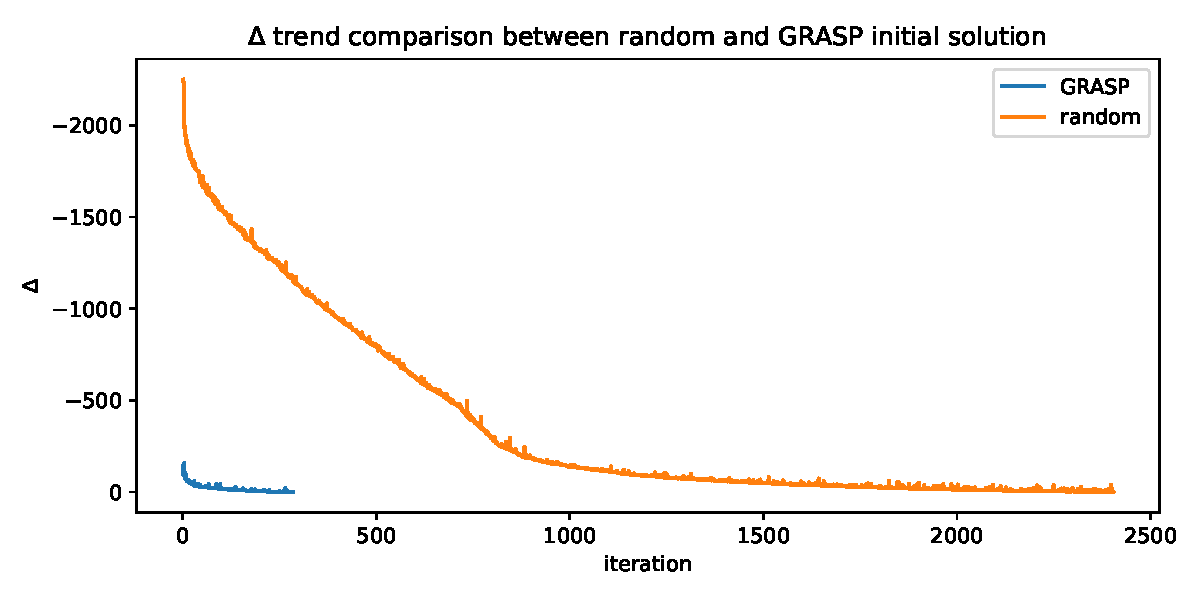
\includegraphics[width=0.78\textwidth]{figures/delta_trend}
    \caption[$\Delta$ trend for different initial solution]{\centering $\Delta$ trend for
    different initial solution. Notice that it's not monotonic}
\end{figure}

This represent the typical trend of $\Delta$ for an instance centered in a 1000
x 1000 box (that explain $\Delta$ in absolute values) for the first downhill.
Future downhills and climbings are similar in the sense that both of them
occupies just few iterations each. Using a GRASP as feeder for an initial
solution (blue line), it's rare to encounter costly crossing (initials are
typically $\sim-100$) and $\Delta$ drops very quickly ($\Delta < 1$ in $\sim250$
iterations). For a random start the situation is different (orange line):
initial $\Delta$ could be very high and there's a typical linear drop followed
by a logarithmic one until no more moves are possible. This typically takes 10
times the iterations using GRAPS as initial solution. For that reason, we will
feed the algorithms using the best GRASP solution among 500 starts, so more time
will be spent on the object in analysis: metaheuristic.\\ One could reply by
saying that our future analysis will be bias against GRASP-ish solutions. Well,
we can't really argue against that, only partially. One could assert that among
the near-optimal solutions, GRAPS don't produces the best ones, even if refined.
We have to remind that refinement could change lot of tour structure and, in
general, don't produce the optimal one, just a very good one. So there is no way
to think that a initially random-refined solution will be better than a
GRAPS-refined one. This justifies the choice of GRAPS among all the constructive
heuristics presented when dealing this kind of situations.\\ 
Another possible degree of freedom in Tabu Search implementation lies in the
tabu list. We keep the things as simple as possible, by tracking the iteration
number when the nodes were marked as tabu and compare it with the actual one: if
the difference is less than the tenure, the nodes is still tabu. There's no need
to implement an actual list, just an array of time stamps.\\
The last point is how to deal the neighborhood size while searching for
solutions. In this case the tenure play the same role as the kick strength in
VNS: by letting it change it's possible to define two phases:
\emph{intensification} and \emph{diversification}. In the first one the tenure is
kept high and lots of nodes will be marked as tabu: there's a small degree of
freedom and new solution will be very similar to the actual one. In the second
one, in which the tenure is small, few nodes will be blocked and there's the
possibility to find very different solutions. A switch between this two phases
is beneficial. The tenure values as well as the phases length are chosen
according to the number of nodes for the first one and according to the time
limit for the second one: we let switch between the phases around two/three
dozen of times during computation.

\section{Genetic algorithm}
The \emph{genetic algorithm} is one of the most popular metaheuristic
techniques. It is widely used in operation research and optimization problem
and it inspired by the natural selection. The idea behind the algorithm exploit
the possibility to merge two different elements of a population to create a new
one that hopefully combines the best characteristic of both parents generating
a better element. For this purpose, when a problem is defined, it is necessary
to establish a measure of performance that in our case is intrinsic considering
we are dealing with an optimization problem. 

The process usually follows the same steps. First of all, a population of $n$
candidate solutions to the problem is generated with a significant randomness
component since diversity is a fundamental feature. Then, a percentage of these
candidates is paired: they returns a new child solution from each pair combining
their chromosome, a data structure containing main information of the solution.
These children are inserted in the population and now among all the candidate
solutions some of them are discarded (\emph{killed}) to keep the population
constant. This series of operations are performed in what is called
\emph{epoch}.\\
By applying a random killing process and a random children procedure there's no
reason to think that the population will improve in terms of cost or, to be
more precise, in term of \emph{fitness}, which is defined as the capacity to
adapt to the environment. Anyway, in our context is simply the cost of a
solution, but this can be adapted to take into account additional constraints.
For this reason, some killing strategies will be discusses and, in addition to
this, \emph{mutations} will be added after children generation: random
improvement of certain solutions. For evolutionary reasons, the best candidate
among epochs, the \emph{champion}, will see its cost decrease, and it will be
returned after the process.

\begin{algorithm}[H]
\SetAlgoLined
\KwResult{An approximated solution}
    \emph{population} $\leftarrow$ n random solutions\;
    \While{time limit is not reached}{
        sample 2k \emph{parent} solution from \emph{population}\;
        \ForEach{pair p} {
            \emph{population} $\leftarrow$ add p \emph{child}\;
        }
        \emph{population} $\leftarrow$ mutate(population)\;
        \emph{population} $\leftarrow$ kill(population)\;
    }
    \emph{sol} $\leftarrow$ best candidate in \emph{population}
    \caption{Genetic Algorithm}
\end{algorithm}

\subsection{Implementation details}
In genetic algorithms implementation choices are mostly based on how solutions
are randomly generated, how they are map into a chromosome and how chromosomes
are combined. In case of TSP the most straightforward way to represent a
solution is an array of length $n$ nodes representing the order in which nodes
are visited. Those instances are created as a random permutation of the nodes.
Anyway, we decided to include very few GRASP solution (generated after just one
start, so they can be not so good). In our tests this speed-up the process
especially in initial epochs.\\
To combine two chromosome they are both split in left and right part. Child left
part is the same of parent 1. Then, all the unvisited nodes of the right part of
parent 2 by the child are added. In this way the child could not visit all the
nodes: the child generation procedure ends with an application of extra-mileage
algorithm to complete the solution and since it's a $\mathcal{O}(n^3)$
operation, this could drive the performances of the whole metaheuristics. In
fact, even if in our tests in the majority of cases only few nodes are left to
visit, in some cases that number could grow to $\sim\nicefrac{3}{8}$ of the total
number of nodes, and that could be costly. One normally should include a
refinement procedure to the child generated, but we decided to skip this
process. As we seen in Tabu Search section, the application of a complete
$2$-opt refinement to a random (or near-random) instance could be costly: we
decided to perform more epochs instead of spending time on this.\\
The mutation procedure is performed using $2$-opt moves on a certain number of
elements of the population. To balance the cost of the operation, we decided to
apply just very few moves to lots of members ($\sim$ 30\% of total population):
in this way we improve a lot the average fitness because, as we show in $\Delta$
trend graph, just few moves applied to a random solution are sufficient: we
decided to apply few dozen of $2$-opt moves, that corresponds to the $\Delta$
before the linear part of the trend.\\
The killing process is not random. One could be tempted to kill the worse
solutions, but they are still useful because they could act as a kick (in VNS
terms), so they could provide interesting and beneficial sub paths for the entire
population. Instead of that, one could analyze the fitness of the population and
do some statistics about that. Our implementation is simpler: we just keep away
from killing process some of the best solution ($\sim$ 20\% of total
population), among the rest of the population
the solutions to be killed are taken at random.\\
To improve even more the best champion found among epochs, we decided to spent some final
time by performing $2$-opt refinements on it.

\section{Metaheuristics comparison}
In this last section we're going to test the three metaheuristics presented,
including the $2$-opt multi start since it's a nice competitor of those. We
tested against 20 instances of 2000 nodes. We tested the
objective as well as how fast they reach it.

Genetic algorithm performances are quite variable, in the sense that certain
runs are comparable with the others metaheuristic, and in some other it cannot
reach good results. This is clear due to the randomness present in each step of
the process. The parameters tuning is performed to try to avoid this kind of
variabilities, but seems unavoidable, at least when the time limit is too low to
let the population reach good average fitness. Anyway, genetic algorithm can be
competitive in other scenario that we will present later on.\\
For this reason, while analyzing the objective reached at the end of the
process, let's exclude for a moment genetic algorithm.

\begin{claim}
    While genetic algorithm's variability makes him not competitive in terms of
    objective, $2$-opt multi start and tabu search are the best ones (even the
    last is more robust), followed by VNS.
\end{claim}

\newpage
\begin{figure}[h!]
    \centering
        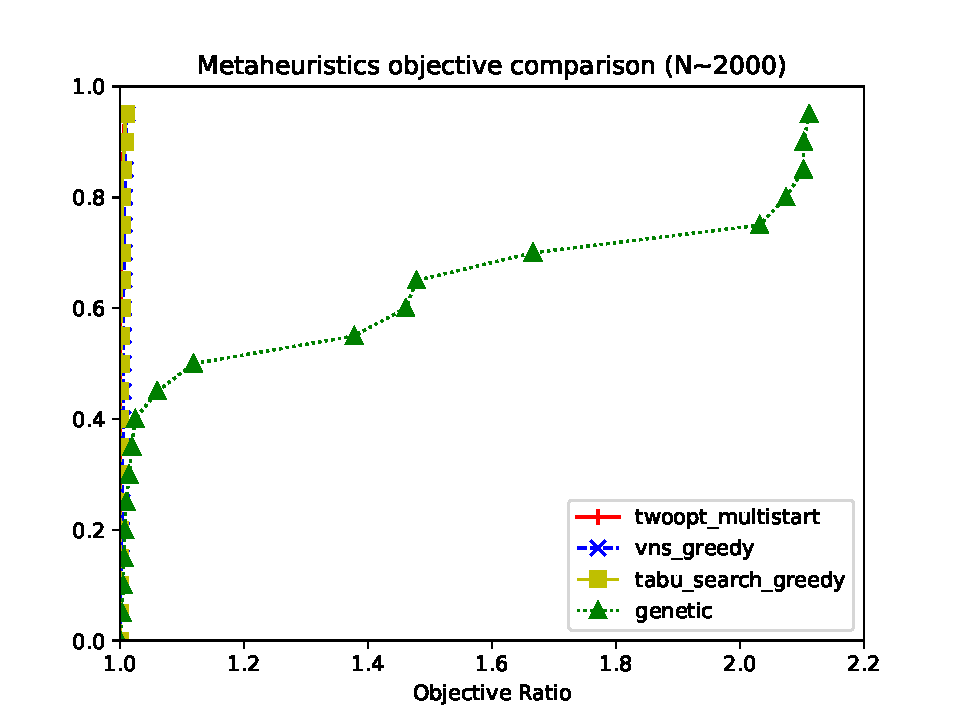
\includegraphics[width=0.8\linewidth]{figures/meta_results.pdf}
        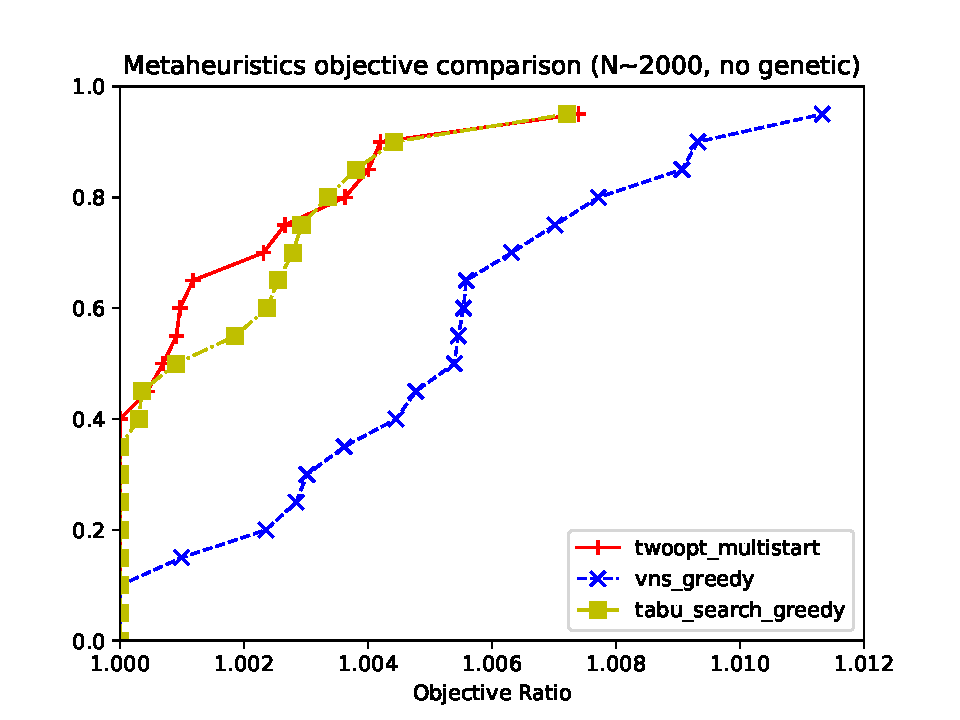
\includegraphics[width=0.8\linewidth]{figures/meta_results_wogenetic.pdf}
        \caption[Metaheuristics objective comparison]{Metaheuristics objective comparison (bottom: genetic algorithm excluded)}
\end{figure}


All of the left three approaches are quite good (the ratio on bottom graph is
pretty low) but a none of those reached $<3\%$ from the exact solution. VNS seems the
third best one, while both Tabu Search and $2$-opt multi start seems the best
options so far. In the case of $2$-opt multi start, that achieves slightly better
results compared with Tabu Search, the multi start approach helps a lot but on
this we noticed some variability that is not present in Tabu Search, that looks
like more robust since it works on an single initial solution: in low time limit
scenario, that would be our choice if one wouldn't take the risk to bet, even if
on average works pretty well.\\

For the last comparison, we solved to optimality the same instances and computed
the exact moment when the objective reached 5\%, 10\%, 50\% from the optimal
solution. This one is a comparison between times that makes possible to analyze
the speed over convergence.\\

\begin{claim}
    Overall, Tabu Search is the fastest algorithm to reaches low
    percentages from optimality. VNS is the second best choice but only if we
    restrict on higher percentages: it slow to achieve near-optimal
    solutions. $2$-opt multi start and genetic algorithm are competitive only at
    low percentages.
\end{claim}

\begin{figure}[h]
    \centering
    \begin{minipage}{.50\textwidth}
        \centering
        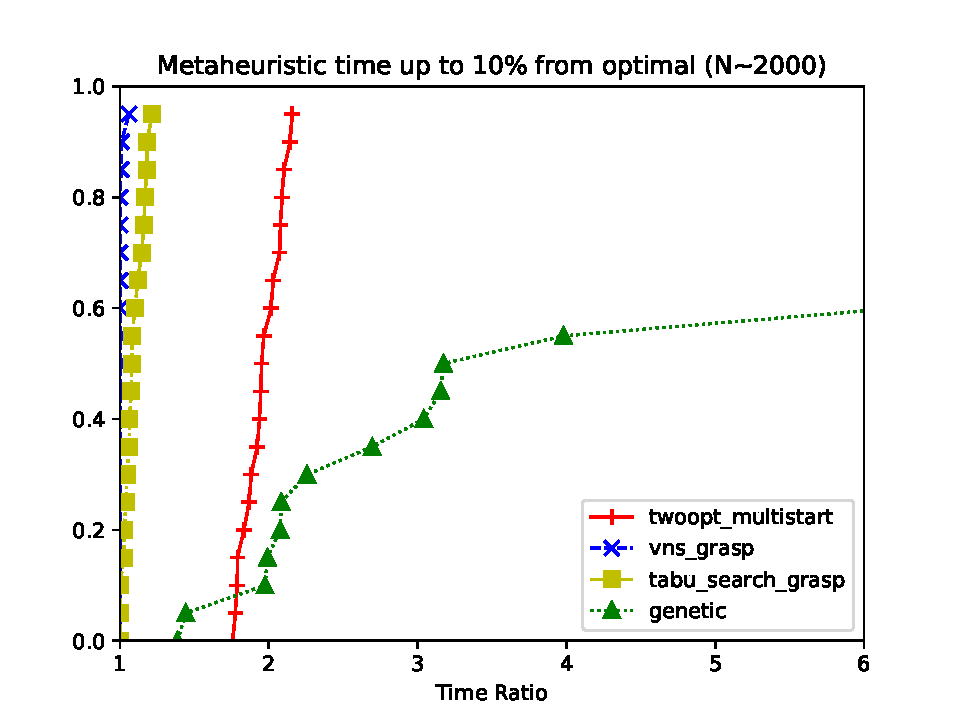
\includegraphics[width=\linewidth]{figures/meta_10.pdf}
    \end{minipage}%
    \begin{minipage}{.50\textwidth}
        \centering
        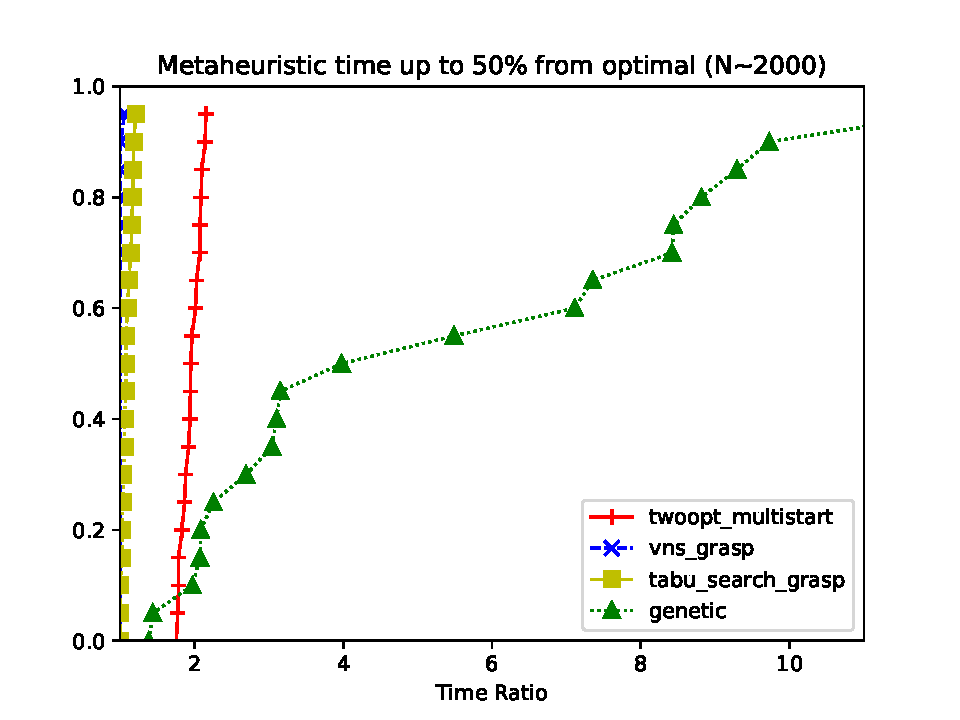
\includegraphics[width=\linewidth]{figures/meta_50.pdf}
    \end{minipage}
    \caption[Metaheuristics time to 10\% and 50\% from optimality
    comparison]{\centering Metaheuristics time to 10\% (left) and 50\% (right) from optimality
    comparison}
\end{figure}


\begin{figure}[h]
    \centering
        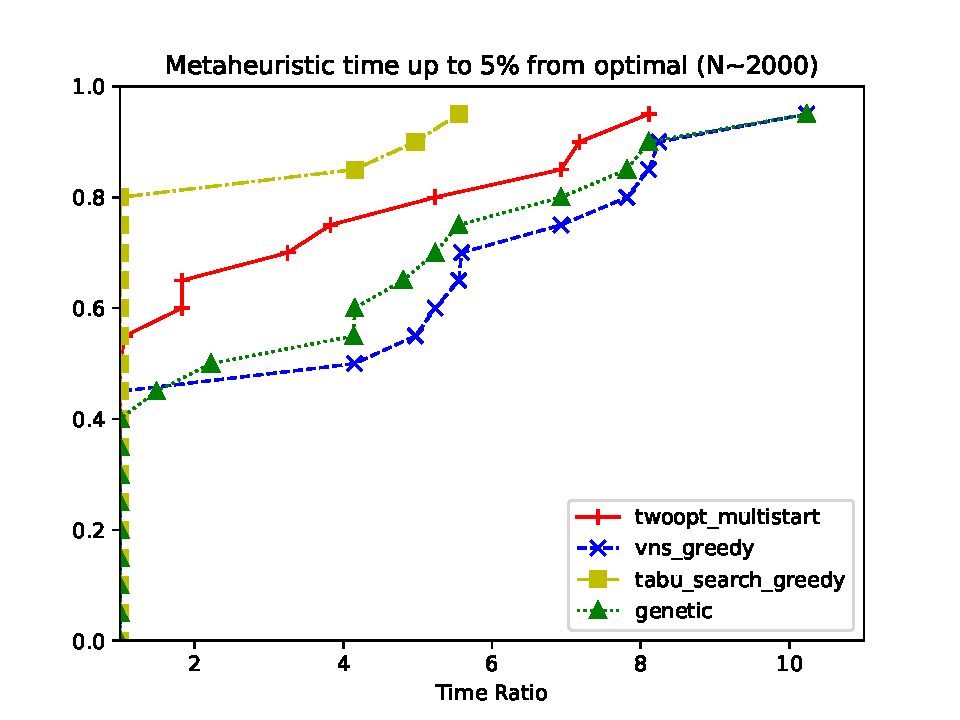
\includegraphics[width=0.75\linewidth]{figures/meta_5.pdf}
    \caption{\centering Metaheuristics time to 5\% from optimality
    comparison}
\end{figure}

Tabu Search is the winner of this round, it's fast to achieve both near-optimal
and more distant solution.\\

We have to state that the analysis of 10\% and 50\% are biased against the
initial starting solution obtained with GRASP in both Tabu Search, VNS and
$2$-opt that share the same analysis in those cases. We can observe that a
initial GRAPS-refined solution is not enough to obtain 50\% from optimal: in
those case, on average, the trend of the three methods should be exactly the
same because the first downhill should be  the same. Let's now suppose that both
shares the first downhill as well as the first local optimum and that a <50\%
solution can be obtained as the second local optimum encountered. Based on the
trends we observed during all the tests done we're now trying to guess the three
behaviours: \begin{itemize}
    \item $2$-opt multi start: after a shared first downhill, an $\epsilon$-cost
        restart is preformed followed by longer, and costly, downhills (and
        restarts) until the second local optimum
    \item VNS: after a shared first downhill, an $\epsilon$-cost
        \say{restart} is preformed by a kick, that move the solution near the
        last one, followed by a shorter downhills (and kicks) until the second
        local optimum
    \item Tabu Search: after a shared first downhill, very short climbing and
        downhills will follows until the second local optimum
\end{itemize}
For reaching 10\% and 50\% solutions, VNS (immediately followed by Tabu Search)
seems the best approach. For reaching near-optimal solution, instead, Tabu
Search is the best, followed by $2$-opt multi start that becomes competitive
because lots of restarts allows it to obtain a very good initial one.\\

Genetic algorithm, for it's nature, does not follow the same trends and, as we
know, starts badly but in the long run seems to achieve very good results due to
the recombination of better and better solutions. In obtaining <5\% solutions,
it's even faster than VNS. In other tests, seems very competitive with a prolonged time limit. 


% Conclusions
% \chapter{Conclusions}
% ...

\appendix
\chapter{Appendix}
\label{appendix:testenv}

All the test we presented were carried out in a protected environment, in order
to avoid performance fluctuation due to system load. A 8 GB RAM machine running
ArchLinux has been prepared, with a idle memory usage of 300 MB (base system and
OpenSSH server). The processor is an Intel i5-6200U, 2 core and 4 threads due to
HyperThreading, with a processor base frequency of 2.30 GHz. The Linux processor
scheduler is ondemand. We noticed in our tests possible thermal throttling, that
should not affect general performances.

NEOS Server
\citep{czyzyk1998neos}


\printReferences

\end{document}
